\documentclass[11pt]{article}

% ---------------------------------------------------------------- packages
\usepackage[utf8]{inputenc}
\usepackage[T1]{fontenc}
\usepackage[margin=1in]{geometry}
\usepackage{graphicx}
\usepackage{booktabs}
\usepackage{amsmath}
\usepackage{amssymb}
\usepackage{caption}
\usepackage{subcaption}
\usepackage{xcolor}
\usepackage[hidelinks]{hyperref}
\usepackage{natbib}
\usepackage{enumitem}

\graphicspath{{../results/figures/}}
\captionsetup{font=small}

\title{\textbf{Content-Based Phishing Detection with an Emphasis on\\
Adversarial Robustness and Explainability}}
\author{Student A --- Content / NLP Detector\\
\small Data Science \& Cyber}
\date{}

\begin{document}
\maketitle

% ================================================================ abstract
\begin{abstract}
\noindent
Phishing e-mail remains a leading entry point for attacks, and much of the signal lives
in the message \emph{text}. This project builds a content-only phishing detector with a
classical NLP pipeline (TF--IDF features with Naive Bayes and Logistic Regression) and
studies it along three axes: detection quality, explainability, and --- the main focus ---
robustness to text-obfuscation evasion. On \textsc{ceas\_08}, the one large corpus with
both classes from a single source, the task is easy on clean text (Logistic Regression F1
$0.998$); but we treat that near-perfect score as a property of clean, single-corpus data
--- not a claim about the wild --- and the rest of the work is a deliberate arms race that
tests when it holds. A word-only model is \emph{fragile}: an imperceptible homoglyph attack
drops recall from $0.99$ to $0.71$. Character n-grams and a Unicode-normalisation defence
restore it and even repair an \emph{unseen} full-width attack, but an adaptive,
importance-guided attacker still opens a residual gap (union $0.99\rightarrow0.87$). We then
close the character front with a \emph{proof}: folding through the full Unicode confusables
set (UTS~\#39) makes the prediction certifiably invariant to that attack family. Honest
evaluation shows the laboratory number survives neither a change of corpus (F1
$0.998\rightarrow0.37$) nor time (a 2008 model catches $14\%$ of real 2023--2025 phishing);
\emph{evolving} the detector on modern mail lifts that to $0.98$ with no forgetting. Pushing
into the next attack class, a word-level \emph{dilution} attack still evades the model
($\rightarrow0.13$), which we answer with a second, orthogonal certificate: a monotone
(non-negative-weight) model provably cannot be un-flagged by inserted text, at an honest
cost of clean F1 $0.998\rightarrow0.912$ --- a certified safety net, not a replacement. We
also test the detector as part of a deployed system: one simulated user report protects the
rest of a phishing campaign, and an LLM-paraphrase probe (validated by a second LLM) leaves
the main model unmoved. Every headline number carries a bootstrap confidence interval, and
classifiers are compared with McNemar's test. Throughout, where a defence is incomplete we
say so --- which is the core argument for fusing this content channel with a second,
independent (URL/sender) detector.
\end{abstract}

% ================================================================ intro
\section{Introduction}

Phishing is a social-engineering attack in which a message impersonates a
trustworthy sender to trick the recipient into revealing credentials, transferring
money, or running malware. It is not a niche problem: phishing is consistently
reported as one of the top initial-access vectors in real breaches, and e-mail is
its main delivery channel. Because so much of the deception is carried by
\emph{language} --- urgency (``your account will be suspended''), authority
(``security team''), and calls to action (``verify now'') --- natural language
processing is a natural tool for detecting it.

This project is the \emph{content} half of a two-part detector. Our job is to read
only the subject and body of an e-mail and decide phishing vs.\ legitimate; a
partner detector (Student B) looks at URLs and sender metadata, and the two are
later combined. Keeping the split clean matters, so we deliberately strip URLs out
of the text (Section~\ref{sec:method}) --- a content model should earn its score
from language, not from links.

Two properties beyond raw accuracy drive the project. First, \textbf{explainability}:
in a security operations centre an analyst needs to know \emph{why} a message was
flagged, not just that it was. Second, and most importantly, \textbf{robustness}.
Spam and phishing filters have been in an arms race with attackers for decades, and
a favourite evasion trick is to mangle the text --- writing \texttt{v\'{e}rify} with a
look-alike character, or \texttt{cl1ck} in leetspeak --- so that a human still reads
the word but a keyword filter does not. A detector that is excellent on clean mail
but falls over on trivially obfuscated mail is not much use.

\paragraph{Contributions.} This is an empirical study, not a new method, and its value is
in rigour and honesty. (1) A \emph{confound-controlled} measurement of lexical detection on a
single mixed-class corpus, with a careful robustness study that separates \emph{seen},
\emph{held-out}, and \emph{adaptive} attacks so a defence is never tested against its own
inverse. (2) An \emph{arms race} in which each defence provokes a smarter attack: character
n-grams and normalisation answer homoglyph obfuscation, an importance-guided attacker lowers
the ceiling, and a principled UTS~\#39 canonicaliser then closes the character front with a
\emph{certified} invariance guarantee. (3) \emph{Honest external validity}: the in-corpus
number survives neither a change of corpus (F1 $0.998\rightarrow0.37$, which we diagnose as
prior-shift plus vocabulary gap) nor time (a 2008 model catches $14\%$ of real 2023--2025
phishing), and \emph{evolving} on modern mail recovers it to $0.98$. (4) A second attack class
--- word-level \emph{dilution} --- answered by a \emph{second, orthogonal certificate}: a
monotone model that cannot be un-flagged by inserted text, with its clean-accuracy cost and
feature-order assumption stated plainly. (5) The detector examined \emph{as part of a deployed
system}: user-report campaign propagation (with the character obfuscation and poisoning risks
it inherits), an LLM-paraphrase probe validated by a second LLM, and a measured deployment
envelope. Throughout we replicate two classical results (Complement NB under imbalance; lexical
fragility to visual attacks), report bootstrap confidence intervals and McNemar tests, and
state every incomplete defence as such.

% ================================================================ background
\section{Background and Literature Review}

\paragraph{Classical spam/phishing filters.} The statistical approach to junk mail
goes back to \citet{sahami1998bayesian}, who framed spam filtering as Naive Bayes
text classification. \citet{metsis2006spam} systematically compared Naive Bayes
variants for spam and is a useful template for the model comparison we run in
Section~\ref{sec:models}. These methods are fast and interpretable and remain
strong when the signal is lexical, but they treat text as a bag of words and are
therefore blind to word order and brittle to obfuscation. Phishing-specific work
such as PILFER \citep{fette2007learning}, the comparison of
\citet{abunimeh2007comparison}, and the filtering approaches of
\citet{bergholz2010new} added engineered features (URL structure, HTML, header
anomalies). Those features are powerful but age quickly and are exactly the signals
our content-only detector deliberately ignores. A recent systematic review of NLP
for phishing e-mail is given by \citet{salloum2022systematic}.

\paragraph{Features and their robustness.} Character n-grams have long been used for
robust text categorisation \citep{cavnar1994ngram}, and character-level models were
shown to be effective for text classification by \citet{zhang2015character}. This is
directly relevant: we find that character n-grams are far more resistant to
obfuscation than word features, because \texttt{cl1ck} still shares letter-chunks
with \texttt{click}.

\paragraph{Adversarial NLP.} The idea that small, human-imperceptible perturbations
can flip a classifier comes from the adversarial-examples literature
\citep{goodfellow2015explaining}. In text, character-level attacks such as
DeepWordBug \citep{gao2018deepwordbug}, TextBugger \citep{li2019textbugger}, and
HotFlip \citep{ebrahimi2018hotflip} evade classifiers by inserting typos and
look-alike characters, while keeping the text readable --- the same
\emph{perceptibility constraint} we adopt. \citet{boucher2022bad} show that
imperceptible Unicode tricks break real, deployed NLP systems, which is our
motivation for taking homoglyphs seriously rather than as a toy. On the defence
side, \citet{eger2019viper} (VIPER) study \emph{visual} attacks and shielding, and
\citet{pruthi2019combating} defend against adversarial misspellings by normalising
text before classification --- the same strategy we use, though we use a rule-based
normaliser derived from the Unicode security data \citep{unicode2023tr39} rather
than a learned word-recogniser. Our robustness experiments (Section~\ref{sec:robust})
are a scoped, methodologically tightened replication of the VIPER attack/shield idea
on phishing e-mail.

\paragraph{Additive attacks and provable defences.} A separate and older evasion strategy does not
disguise the message at all: it \emph{adds} innocuous content until the classifier's summed evidence
tips the other way. \citet{lowd2005good} formalised this as the \emph{good-word attack} on statistical
spam filters, showing that appending enough common benign words pushes a large share of blocked spam
past the filter --- our dilution attack (Section~\ref{sec:wordattack}) is an instance of it, which we
rediscovered empirically before connecting it to this literature. Defences have mostly been heuristic:
\citet{jorgensen2008multiple} counter it with multiple-instance learning over message segments.
A stronger option is to make the attack impossible rather than unlikely --- \citet{fleshman2018nonnegative}
show, for malware, that constraining a model to non-negative weights means added features can only
increase the maliciousness score, so evasion requires \emph{removing} malicious content. We adopt that
construction for phishing text in Section~\ref{sec:monotone}, and---because a certificate is only
meaningful next to its price---measure what the constraint costs in clean accuracy.

\paragraph{Transformers.} Self-attention \citep{vaswani2017attention} and BERT
\citep{devlin2019bert} model word order and context that bag-of-words ignores.
DistilBERT \citep{sanh2019distilbert} is a smaller, faster distillation we use as a
transformer baseline. We report Matthews Correlation Coefficient throughout because,
as \citet{chicco2020advantages} argue, it is more informative than F1 or accuracy on
imbalanced binary problems.

\paragraph{Where this project sits.} Most phishing-NLP work reports clean accuracy.
Comparatively little reports robustness to cheap character obfuscation
\emph{evaluated against attacks the defence has not seen}, and fewer still quantify
what that robustness costs in interpretability. That gap is what this project
targets.

% ================================================================ methodology
\section{Methodology}
\label{sec:method}

\subsection{Data and the corpus-confound problem}
We use the Kaggle ``Phishing Email Dataset'' compilation \citep{alam2023phishing},
which ships several classic corpora as separate labelled CSVs. A subtle danger with
such compilations is \emph{corpus confounding}: if all phishing came from one corpus
(e.g.\ Nazario) and all legitimate mail from another (e.g.\ Enron), a classifier
could score highly just by recognising \emph{which corpus} a message came from,
learning nothing about phishing. We demonstrate this directly in
Section~\ref{sec:probe}. To avoid it, all main experiments use a single corpus,
\textsc{ceas\_08}, which is the only large corpus in the pack that contains
\emph{both} classes from the same source; the confound is then impossible by
construction.

Two deliberate preprocessing choices follow. (1) \textbf{URLs are stripped} from the
text and replaced by a \texttt{URL} token, so the content model cannot ride on the
link signal that belongs to the partner detector. (2) We \textbf{rebalance to a
legit-majority base rate} (35\% phishing). Real inboxes are mostly legitimate, and
--- as Section~\ref{sec:robust} shows --- a phishing-majority prior actually
\emph{hides} evasion attacks: a model that loses its signal falls back to the
majority class, so if that class is ``phishing'' the attack looks harmless. The
working set has $26{,}633$ e-mails; a SHA-256 hash of the frozen snapshot is written
alongside the results for reproducibility.

\subsection{Features and feature engineering}
\label{sec:featureng}
Each e-mail (subject $+$ body) becomes a \textbf{TF--IDF} vector: Term Frequency counts a
term's occurrences, Inverse Document Frequency up-weights rare, discriminative ones such as
``verify account''; \texttt{sublinear\_tf} log-scales the counts so a word repeated fifty
times cannot dominate. We compare three configurations --- \textbf{word} (1--2 grams,
stop-words removed), \textbf{char} (character 3--5 grams, \texttt{char\_wb}), and their
\textbf{union} --- because character n-grams capture sub-word shape and, as we will see,
resist obfuscation. \texttt{min\_df} and \texttt{max\_features} drop ultra-rare tokens and
cap the vocabulary; no scaling is needed (TF--IDF vectors are L2-normalised). We deliberately
avoid dimensionality reduction (e.g.\ Truncated SVD): it would blur the one-token-one-weight
interpretability of Section~\ref{sec:explain}, and the linear model already handles the sparse
high-dimensional space well.

\paragraph{Redundancy.} Redundancy appears in two places. Among the interpretable
meta-features (Section~\ref{sec:corr}), message length and word count are almost
perfectly rank-correlated ($\rho \approx 0.97$) and carry a variance inflation factor of
$\approx 21$ each, so using both as inputs would split their importance across
near-duplicates. In the model, a word and its character n-grams encode overlapping
information about the same token; harmless for accuracy but it dilutes explanations. We
spot such redundancy with rank correlation and VIF and, for the model, by treating the
coarse meta-features as diagnostics rather than inputs.

\subsection{Models}
\label{sec:models}
Naive Bayes applies Bayes' theorem with the ``naive'' assumption that features are
conditionally independent given the class:
\[
P(y \mid \mathbf{x}) \propto P(y)\prod_i P(x_i \mid y).
\]
\textbf{Laplace (add-one) smoothing} solves the \emph{zero-frequency problem}: if a
word never appeared in one class during training, we do not want a single unseen
word to zero out the whole class probability. \textbf{Complement Naive Bayes}
\citep{rennie2003tackling} is a variant designed to behave better under class
imbalance, which we test rather than assume (Section~\ref{sec:imbalance}). We compare
Multinomial NB, Complement NB, and \textbf{Logistic Regression} (an interpretable
linear baseline). Model selection uses validation F1; the test set is touched once.

\subsection{Evaluation and statistics}
\label{sec:metricdef}
We report accuracy, precision, recall, $F_1$, $F_2$, MCC and AUC, but weight them
deliberately for an imbalanced security task. Accuracy is reported and not trusted alone:
under a legit-majority base rate a do-nothing model scores high while catching no phishing
(the \emph{accuracy paradox}). Because a false negative (missed phishing) is far costlier
than a false positive (a false alarm), we emphasise \emph{recall}, the recall-weighted
$F_2$ ($F_\beta$ with $\beta=2$), and \textbf{MCC} --- which uses all four confusion cells
and stays honest under imbalance \citep{chicco2020advantages} --- and we pick a cost-optimal
threshold on validation with a miss weighted five times a false alarm. AUC gives
threshold-independent ranking quality, relevant because we move that threshold. For
statistical validity every headline metric carries a \textbf{bootstrap $95\%$ confidence
interval} (1000 resamples), and classifiers are compared with \textbf{McNemar's exact test}
on their paired errors.

\subsection{Threat model and attacks}
\label{sec:threat}
The attacker can edit the e-mail \emph{text} but not our pipeline (test-time
\emph{evasion}). They perturb only the phishing e-mails --- they want those to slip
through --- so we measure \textbf{recall on phishing}. Perturbations are bounded so
the text stays human-readable (homoglyphs are in fact \emph{identical} to the eye).
We distinguish three attack families, which is what makes the defence evaluation
honest:
\begin{itemize}[nosep]
  \item \textbf{Seen} --- homoglyphs (Latin$\rightarrow$Cyrillic) and leetspeak, the
  family the normaliser is built around;
  \item \textbf{Held-out} --- full-width characters, a \emph{different} family the
  normaliser was not tuned for;
  \item \textbf{Adaptive} --- an attacker who knows about normalisation and uses
  confusable letters deliberately absent from the normaliser's table.
\end{itemize}

\paragraph{Where these sit in the standard taxonomy.} In the usual adversarial-ML
vocabulary, everything above is a test-time \emph{evasion} attack of the second kind
(turning a positive/phishing into a negative), never a training-time \emph{poisoning}
attack --- with one exception we return to later: the user-report channel of
Section~\ref{sec:feedback}, where false reports are a genuine poisoning/label-flipping
attack on a model that learns from feedback. Our attacks span the specificity axis too:
the uniform perturbations are \emph{indiscriminate}, while the importance-guided attack of
Section~\ref{sec:targeted} is \emph{targeted}, spending its budget on the model's
highest-weight tokens. Knowledge-wise it is a \emph{grey-box} attack --- it reads the linear
model's coefficients but not its training data --- and we also test \emph{transferability}
by replaying a lexical attack against DistilBERT (Section~\ref{sec:distilbert}). We do
\emph{not} study \emph{model-extraction}/theft (an attacker cloning the detector through
query access); it is a real risk for a deployed API and we note it as future work rather
than pretend otherwise.

\subsection{Defences}
We evaluate two defences, and they are the two textbook countermeasures for text
obfuscation: \emph{normalise the input}, and \emph{train on adversarial examples}. The
first, \textbf{normalisation}, cleans the text before classification: it maps a curated
table of Unicode confusables back to Latin, applies a generic Unicode (NFKD) fold, strips
invisible characters, lower-cases, de-leets, and collapses in-word separators --- exactly
the ``convert homoglyphs / normalise text'' recipe recommended against these attacks. The table is a practical subset of the Unicode security
data \citep{unicode2023tr39}; it is intentionally incomplete, which is what gives the
adaptive attacker room and lets us measure the defence \emph{ceiling} rather than a
tautological victory. The second, \textbf{adversarial training}
(Section~\ref{sec:advtrain}), instead augments the training set with perturbed copies
of the phishing training emails and retrains, so the model learns the attack directly.
We report both and, importantly, their combination.

% ================================================================ experiments
\section{Experiments and Results}

\subsection{The corpus-confound probe}
\label{sec:probe}
To justify the single-corpus design we trained a classifier to predict which corpus
a phishing e-mail came from (\textsc{ceas}, Nazario, or Nigerian-Fraud). It reached
\textbf{98.8\%} accuracy against a 33\% chance baseline: the corpora are trivially
separable by provenance. Pooling single-class phishing corpora with a separate ham
source would therefore let a ``detector'' cheat, which is exactly why the main
experiments live inside \textsc{ceas\_08}.

\subsection{Exploratory analysis and trivial baselines}
The corpus is clean (almost pure ASCII; a median non-ASCII share near zero), which
is the backdrop against which the later attacks stand out. Two dumb baselines set
the scale (Table~\ref{tab:baselines}). A \emph{majority} classifier scores 65\%
accuracy while catching \emph{zero} phishing --- the \textbf{accuracy paradox} in
one line --- and a small keyword list does little better (F1 $0.25$, MCC slightly
negative). Real models must beat these, not just the 50\% coin-flip.

\begin{table}[t]
\centering
\caption{Trivial baselines on the test set. The majority classifier illustrates the
accuracy paradox: high accuracy, no detection.}
\label{tab:baselines}
\begin{tabular}{lcccccc}
\toprule
 & Accuracy & Precision & Recall & F1 & MCC & AUC \\
\midrule
Majority (all legit) & 0.650 & 0.000 & 0.000 & 0.000 & 0.000 & 0.500 \\
Keyword list         & 0.556 & 0.304 & 0.208 & 0.247 & $-0.054$ & 0.476 \\
\bottomrule
\end{tabular}
\end{table}

\subsection{Exploratory data analysis of interpretable meta-features}
\label{sec:corr}
Because TF--IDF is too high-dimensional to correlate token-by-token, we engineered a
handful of interpretable meta-features (length, word count, digit / uppercase /
non-ASCII ratios, URL-token count) and analysed them with the standard EDA toolkit:
distribution shape, a rank correlation, a redundancy diagnostic, and a hypothesis test.
The aim is not to add model inputs --- the lexical model already saturates --- but to turn
each downstream methodological choice into a \emph{tested} statement rather than an
assumption.

\paragraph{Distribution shape decides the right statistics.} We first measured the
\textbf{skewness} (asymmetry) and \textbf{excess kurtosis} (tailedness) of each feature
(Table~\ref{tab:edashape}). The ratio features are strongly right-skewed and heavy-tailed
--- average word length has skewness $\approx 6.6$ and excess kurtosis above $60$, digit
ratio skewness $\approx 3.2$ --- so they are nowhere near normal. This is precisely why
\textbf{Spearman} rank correlation (and the \textbf{median}, not the mean, for central
tendency) is the correct tool: it measures monotonic association without Pearson's
normality/linearity assumptions, and it is robust to the heavy tails, while Kendall's
$\tau$ targets smaller samples than our tens of thousands of rows. Character length looks
only mildly skewed here \emph{because} every e-mail is truncated at \texttt{MAX\_CHARS}
during preprocessing, which caps the long right tail by construction --- a choice that
doubles as outlier control, so a robust IQR/MAD outlier scan on the truncated length flags
essentially nothing.

\paragraph{Length is the clearest signal --- and we test it.} On the Spearman heat-map the
clearest signal is \textbf{length}: phishing e-mails are \emph{shorter} than legitimate
ones ($\rho \approx -0.57$ for characters, $-0.53$ for word count), matching the intuition
that a scam is a short, urgent message while legitimate mailing-list traffic is long and
threaded. Rather than leave this at an eyeballed histogram, we test it: the phishing median
length ($\approx 290$ characters) is far below the legitimate median ($\approx 1{,}185$),
and because the distributions are skewed we use the non-parametric \textbf{Mann--Whitney
$U$} test, which rejects the null of equal distributions at $p \ll 0.001$. Yet even the
strongest meta-feature is only a moderate correlation --- far from the near-perfect
separation the lexical model achieves --- confirming that the real signal is \emph{which
words appear}, not coarse surface statistics.

\paragraph{Redundancy, quantified.} Length and word count are visibly collinear on the
heat-map ($\rho\approx0.97$). We quantify this with the \textbf{variance inflation factor}
(VIF), the standard multicollinearity diagnostic: both features have $\mathrm{VIF}\approx
21$, well past the conventional threshold of $10$, whereas every other meta-feature sits
near $1$--$3$. They encode almost the same information, so feeding both to a linear model
would split one signal across two coefficients and distort any interpretation. This is why
the entire meta-feature block is kept \textbf{diagnostic-only} and never enters the
classifier (Fig.~\ref{fig:eda}).

\paragraph{A data-quality check on the dates.} The corpus's \texttt{date} headers are
$99.7\%$ within the expected 2007--2009 window. We explicitly checked for the classic
Unix-epoch trap --- a \emph{missing} date imputed to $0$ becomes \texttt{1970-01-01} and
would masquerade as a real timestamp in any temporal view --- and found \textbf{none} (0 of
$34{,}342$ emails). The $\approx0.3\%$ of off-window dates are genuinely \emph{spoofed}
RFC-822 headers (implausible years such as $2086$), which the temporal analysis already
excludes, so the single-period snapshot is trustworthy.

\begin{table}[t]
\centering
\caption{Distribution shape of the interpretable features. Large positive skewness and
excess kurtosis on the ratio features (non-normal, heavy-tailed) are what make a rank-based
correlation and the median the correct choices.}
\label{tab:edashape}
\begin{tabular}{lccc}
\toprule
feature & median & skewness & excess kurtosis \\
\midrule
length (chars)     & 800  & 0.33 & $-1.43$ \\
word count         & 133  & 0.41 & $-1.17$ \\
avg.\ word length  & 5.04 & \textbf{6.56} & \textbf{63.1} \\
digit ratio        & 0.02 & 3.24 & 19.0 \\
uppercase ratio    & 0.05 & 2.68 & 7.2 \\
\bottomrule
\end{tabular}
\end{table}

\begin{figure}[t]
\centering
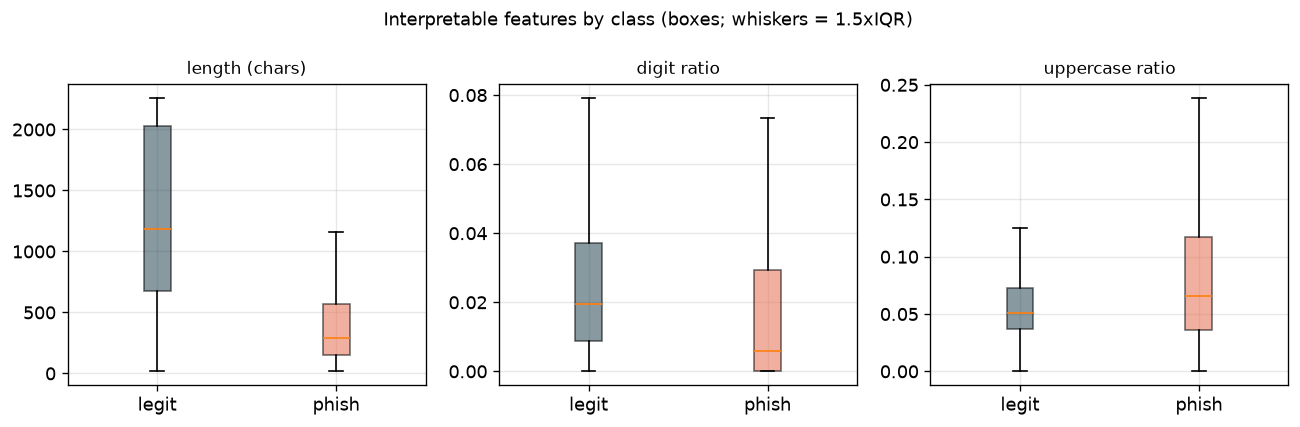
\includegraphics[width=\linewidth]{../results/figures/F13_eda_boxplots.png}
\caption{Interpretable features by class (whiskers at $1.5\times$IQR, outliers hidden for
readability). Phishing e-mail is markedly shorter and slightly more digit- and
uppercase-heavy; the box widths also make the skew of the ratio features visible.}
\label{fig:eda}
\end{figure}

\subsection{Clean detection: features and models}
On clean text the task is easy. All three feature sets give F1 $\ge 0.994$
(Table~\ref{tab:ablation}), with the \textbf{union} best. Among classifiers
(Table~\ref{tab:models}), Logistic Regression clearly wins (F1
$0.998$, MCC $0.997$), and McNemar's test confirms the gap over Complement NB is
statistically significant ($p \ll 0.001$), not luck. Complement NB edges Multinomial
NB, consistent with \citet{metsis2006spam,rennie2003tackling}. The confusion matrix
for the selected model (Fig.~\ref{fig:confusion}) shows only a handful of errors.

\begin{table}[t]
\centering
\caption{Feature ablation with Logistic Regression (clean test set). F1 shown with a
bootstrap 95\% CI.}
\label{tab:ablation}
\begin{tabular}{lccccccl}
\toprule
Features & Accuracy & Precision & Recall & F1 & F2 & MCC & F1 (95\% CI) \\
\midrule
word  & 0.9962 & 0.9968 & 0.9925 & 0.9946 & 0.9933 & 0.9917 & $0.995\,[0.992,0.997]$ \\
char  & 0.9968 & 0.9946 & 0.9962 & 0.9954 & 0.9959 & 0.9930 & $0.995\,[0.993,0.997]$ \\
union & \textbf{0.9985} & 0.9979 & 0.9979 & \textbf{0.9979} & 0.9979 & \textbf{0.9967} & $0.998\,[0.996,0.999]$ \\
\bottomrule
\end{tabular}
\end{table}

\begin{table}[t]
\centering
\caption{Model comparison on union features (clean test set).}
\label{tab:models}
\begin{tabular}{lccccccl}
\toprule
Model & Accuracy & Precision & Recall & F1 & F2 & MCC & F1 (95\% CI) \\
\midrule
Multinomial NB & 0.9807 & 0.9977 & 0.9469 & 0.9716 & 0.9566 & 0.9577 & $0.972\,[0.966,0.977]$ \\
Complement NB  & 0.9835 & 0.9972 & 0.9555 & 0.9759 & 0.9635 & 0.9638 & $0.976\,[0.971,0.981]$ \\
Logistic Reg.  & \textbf{0.9985} & 0.9979 & 0.9979 & \textbf{0.9979} & 0.9979 & \textbf{0.9967} & $0.998\,[0.996,0.999]$ \\
\bottomrule
\end{tabular}
\end{table}

\begin{figure}[t]
\centering
\begin{subfigure}{0.32\textwidth}
  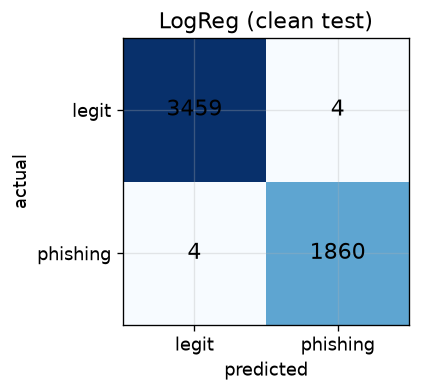
\includegraphics[width=\linewidth]{F3_confusion_clean.png}
  \caption{Confusion matrix (clean).}
  \label{fig:confusion}
\end{subfigure}\hfill
\begin{subfigure}{0.32\textwidth}
  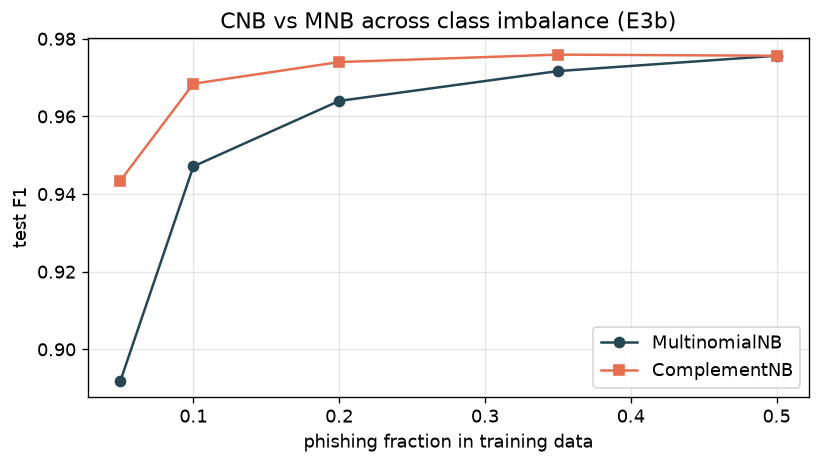
\includegraphics[width=\linewidth]{F_imbalance_sweep.png}
  \caption{CNB vs.\ MNB across imbalance.}
  \label{fig:imbalance}
\end{subfigure}\hfill
\begin{subfigure}{0.32\textwidth}
  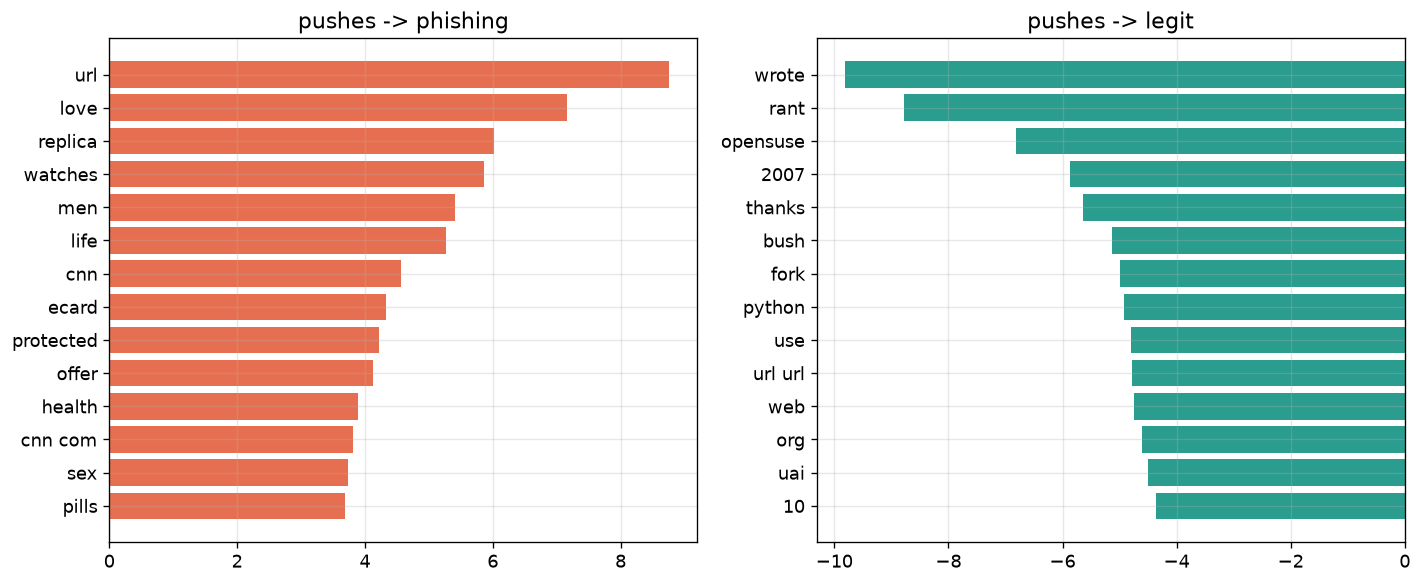
\includegraphics[width=\linewidth]{F4_feature_weights.png}
  \caption{Top signed word weights.}
  \label{fig:weights}
\end{subfigure}
\caption{Clean-data diagnostics.}
\end{figure}

\subsection{Does Complement NB help under imbalance?}
\label{sec:imbalance}
\citet{rennie2003tackling} claim CNB corrects Naive Bayes under class imbalance.
Rather than assert it, we tested it: holding the vectoriser fixed, we retrained MNB
and CNB on training subsets ranging from 5\% to 50\% phishing
(Fig.~\ref{fig:imbalance}). The paper's claim holds on our data --- at 5\% phishing
CNB beats MNB by a clear margin (F1 $0.944$ vs.\ $0.892$), and at a genuine 50/50
balance the gap disappears entirely ($0.976$ vs.\ $0.976$). This is a small but genuine
confirmation of the mechanism, on a different corpus than the original: the advantage is
\emph{specifically} an imbalance correction, and it vanishes exactly where the theory says
it should. Note that above $35\%$ phishing the working set does not contain enough phishing
e-mail to reach the target share by adding positives, so we down-sample the legitimate class
instead; clamping the positive count would silently re-use the $35\%$ subset for every
higher target and manufacture a spurious residual gap at ``balance''.

\subsection{Tuning and generalisation}
A validation-only grid search over the regularisation strength $C$ selected the best
value, with a negligible validation-to-test F1 gap, indicating the model generalises
within the corpus rather than memorising. The cost-optimal threshold ($0.40$, below
the default $0.5$) nudges recall up ($0.9979 \rightarrow 0.9984$) at a tiny precision
cost, reflecting the ``a miss is worse than a false alarm'' asymmetry.

\subsection{Adversarial robustness --- the main result}
\label{sec:robust}
Figure~\ref{fig:money} and Table~\ref{tab:robust} are the centre of the project. On
\emph{clean} text both models catch essentially all phishing. Under an
\textbf{imperceptible homoglyph+leet attack} the \textbf{word-only} model collapses:
recall falls from $0.99$ to $0.71$ --- nearly 30\% of phishing now sails through,
with no visible change to a human reader. Two defences answer it. First, character
n-grams are robust in their own right: the \textbf{union} model only drops to
$0.93$, because sub-word chunks survive letter swaps. Second, \textbf{normalisation}
restores the word-only model to $0.99$.

The honest part is what happens against attacks the defence did \emph{not} target.
Against a \textbf{held-out} full-width attack the undefended word model is just as
fragile ($0.68$), yet normalisation still repairs it to $0.99$ --- not because we
listed full-width characters, but because the defence's \emph{generic} Unicode fold
handles them. This is the good kind of generalisation. But an \textbf{adaptive}
attacker, who uses confusable letters we deliberately left out of the table, keeps
recall down at $0.96$ even after normalisation. The defence helps a lot; it is not a
silver bullet. Figure~\ref{fig:budget} shows the same story as the attack strength is
swept: word-only recall degrades steeply while union stays high.

\begin{table}[t]
\centering
\caption{Recall on phishing under attack and defence (test set). ``+ normalise''
applies the normalisation defence. The word-only model collapses and is repaired; the
adaptive attacker sets the ceiling.}
\label{tab:robust}
\begin{tabular}{lcc}
\toprule
Setting & word-only recall & union recall \\
\midrule
clean                         & 0.992 & 0.998 \\
homoglyph+leet (seen)         & 0.711 & 0.933 \\
\quad + normalise             & 0.992 & 0.998 \\
full-width (held-out)         & 0.677 & 0.920 \\
\quad + normalise             & 0.993 & 0.998 \\
adaptive (unmapped)           & 0.888 & 0.983 \\
\quad + normalise             & \textbf{0.963} & 0.987 \\
\bottomrule
\end{tabular}
\end{table}

\begin{figure}[t]
\centering
\begin{subfigure}{0.48\textwidth}
  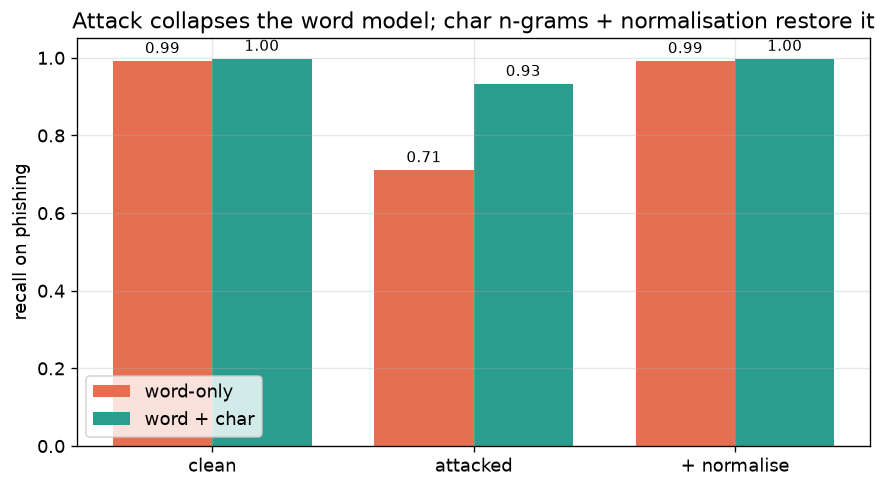
\includegraphics[width=\linewidth]{F5_robustness_bars.png}
  \caption{Clean vs.\ attacked vs.\ defended.}
  \label{fig:money}
\end{subfigure}\hfill
\begin{subfigure}{0.48\textwidth}
  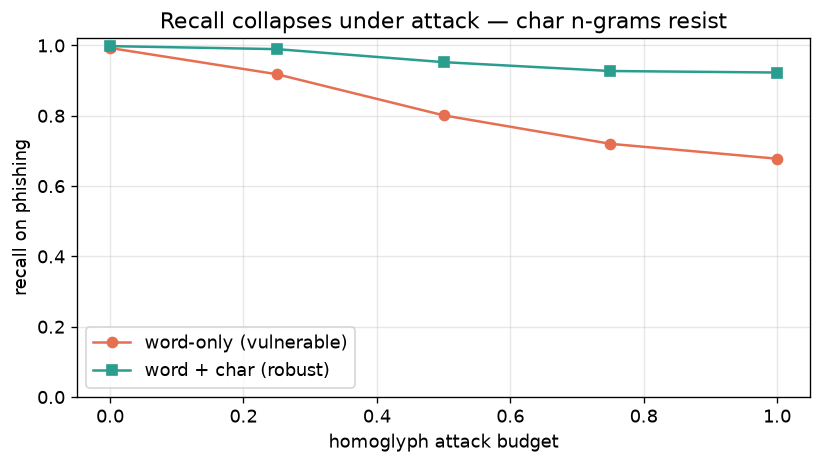
\includegraphics[width=\linewidth]{F7_budget_sweep.png}
  \caption{Recall vs.\ attack budget.}
  \label{fig:budget}
\end{subfigure}
\caption{Adversarial robustness. Word-only features are fragile; character n-grams
and normalisation restore recall, up to the adaptive-attacker ceiling.}
\end{figure}

\subsection{A stronger, importance-guided attacker}
\label{sec:targeted}
The adaptive attacker above perturbs characters \emph{uniformly}. A real adversary
spends its budget where it matters --- on the few tokens the model weights most --- the
classic word-importance attack of DeepWordBug \citep{gao2018deepwordbug}, TextBugger
\citep{li2019textbugger} and HotFlip \citep{ebrahimi2018hotflip} (implemented here in
the spirit of the TextAttack framework \citep{morris2020textattack}). Because our model
is linear, each token's phishing pull is exactly its coefficient, so we rank the words
of every phishing e-mail by that pull and homoglyph only the top $k$.
Figure~\ref{fig:targeted} contrasts this with a random-word attack at the \emph{same}
edit budget: eight \emph{targeted} edits cut word-only recall to $0.74$, whereas eight
\emph{random} edits leave it at $0.98$. A median of just \textbf{9 words}
($\approx$23\% of the letters, all homoglyphs and so invisible to a reader) is enough
to flip a phishing e-mail, and $1{,}090$ of $1{,}864$ phishing e-mails ($58\%$) are
evaded within 25 edits.

More importantly, the targeted attacker lowers the defence \emph{ceiling}
(Table~\ref{tab:ceiling}). The uniform adaptive attacker left the fully-defended union
model at $0.99$; a \emph{targeted} adaptive attacker --- unmapped confusables, spent on
the highest-weight tokens, then normalised --- drops it to $0.87$, and the word model to
$0.67$. This does not overturn Section~\ref{sec:robust}: character n-grams and
normalisation still remove most of the risk. But it shows the residual gap against a
competent, defence-aware adversary is wider than a uniform attack implies --- the
strongest form of the ``no silver bullet'' conclusion, and a concrete measure of the
work a second, independent signal must do.

\begin{table}[t]
\centering
\caption{Defence ceiling under a \emph{targeted} adaptive attacker (unmapped
confusables spent on high-weight tokens, then normalisation), vs.\ the uniform adaptive
attacker of Table~\ref{tab:robust}. Recall on phishing.}
\label{tab:ceiling}
\begin{tabular}{lcc}
\toprule
Attacker (all $+$ normalise) & word recall & union recall \\
\midrule
uniform adaptive (Table~\ref{tab:robust}) & 0.963 & 0.987 \\
targeted adaptive, $k=8$   & 0.836 & 0.955 \\
targeted adaptive, $k=20$  & 0.673 & \textbf{0.879} \\
\bottomrule
\end{tabular}
\end{table}

\begin{figure}[t]
\centering
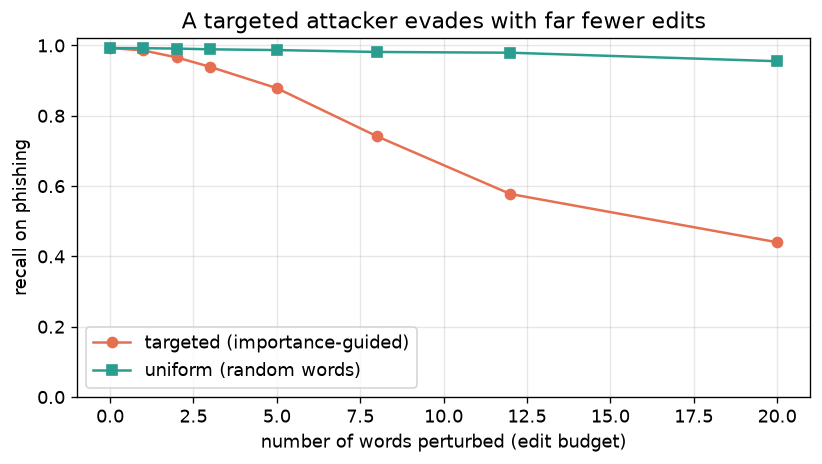
\includegraphics[width=0.6\textwidth]{F12_adaptive_budget.png}
\caption{At a matched edit budget an importance-guided attacker evades far more often
than a random one: targeted recall collapses with a handful of edits while uniform
recall barely moves.}
\label{fig:targeted}
\end{figure}

\subsection{Robustness checks: stability and cost}
\label{sec:ci}
Two honesty checks accompany the main result. \textbf{Stability:} the attacks are
stochastic, so each cell of Table~\ref{tab:robust} is a single draw; repeating every attack
over $K=10$ seeds (Table~\ref{tab:ci}) gives standard deviations of at most a few
thousandths of recall, so the collapse-and-recovery is a genuine effect, not a lucky draw.

\begin{table}[t]
\centering
\caption{Multi-seed robustness ($K=10$ attack seeds): mean $\pm$ s.d.\ of recall on
phishing.}
\label{tab:ci}
\begin{tabular}{lcc}
\toprule
Setting & word-only & union \\
\midrule
homoglyph+leet             & $0.717\pm0.003$ & $0.936\pm0.003$ \\
\quad + normalise          & $0.991\pm0.001$ & $0.998\pm0.000$ \\
full-width (held-out)      & $0.680\pm0.001$ & $0.921\pm0.002$ \\
\quad + normalise          & $0.993\pm0.000$ & $0.998\pm0.000$ \\
adaptive (unmapped)        & $0.884\pm0.004$ & $0.983\pm0.002$ \\
\quad + normalise          & $0.959\pm0.004$ & $0.986\pm0.001$ \\
\bottomrule
\end{tabular}
\end{table}

\paragraph{What the defence costs.} Normalisation is applied to \emph{every} incoming
e-mail, so it must not damage legitimate mail. Normalising the whole clean test set leaves
recall unchanged but raises the union model's false-positive rate from $0.0012$ to $0.0040$
(word-only: $0.0017\rightarrow0.0049$), flipping about a dozen mostly-legitimate e-mails.
The defence is cheap but not free --- a small, quantifiable precision cost on ordinary
traffic, worth stating rather than hiding.

\subsection{Adversarial training: a second, complementary defence}
\label{sec:advtrain}
Normalisation cleans the input \emph{before} the model; \textbf{adversarial training}
does the opposite --- it leaves the input alone and teaches the model about the
attack, by adding homoglyph+leet perturbed copies of the phishing \emph{training}
emails and retraining (only training rows are perturbed, so there is no leakage). The
question is whether hardening against one attack family also helps against families
the model never saw. Table~\ref{tab:advtrain} and Figure~\ref{fig:advtrain} answer it,
and the answer is the classical one \citep{goodfellow2015explaining}: adversarial
training is near-perfect on the family it \emph{was} trained on ($1.00$ on
homoglyph+leet) but \emph{generalises poorly} to a held-out family ($0.78$ on
full-width), because it has memorised particular look-alike characters rather than the
idea of obfuscation. Normalisation is the mirror image: it was not tuned for the
held-out family either, yet its generic Unicode folding still recovers it ($0.99$),
while it is a little weaker against the adaptive attacker. The two defences therefore
cover each other's blind spots, and \textbf{combining them} gives the best recall
across every family ($\ge 0.98$). The practical lesson is that adversarial training
belongs \emph{alongside} a principled input defence, not instead of one.

\begin{table}[t]
\centering
\caption{Word-only recall on phishing: two defences across attack families.
Adversarial training excels on the trained family but not on unseen ones;
normalisation generalises better; together they cover every family.}
\label{tab:advtrain}
\begin{tabular}{lcccc}
\toprule
Attack family & undefended & normalisation & adv.\ training & adv.\ + norm \\
\midrule
clean                  & 0.992 & 0.993 & 0.995 & 0.995 \\
homoglyph+leet (seen)  & 0.711 & 0.992 & \textbf{1.000} & 0.995 \\
full-width (held-out)  & 0.677 & \textbf{0.993} & 0.781 & 0.995 \\
adaptive (unmapped)    & 0.888 & 0.963 & 0.938 & \textbf{0.983} \\
\bottomrule
\end{tabular}
\end{table}

\begin{figure}[t]
\centering
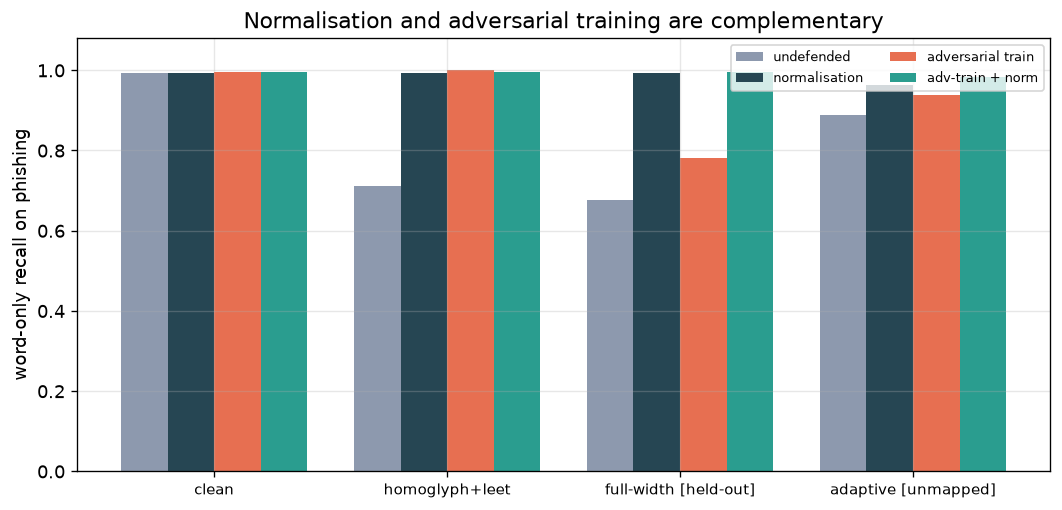
\includegraphics[width=0.7\textwidth]{F8_adversarial_training.png}
\caption{Normalisation and adversarial training are complementary: each is strong
where the other is weak, and combining them is robust across all attack families.}
\label{fig:advtrain}
\end{figure}

\subsection{The arms race: closing the gap the targeted attacker opened}
\label{sec:armsrace}
Section~\ref{sec:targeted} left a wound: an importance-guided adaptive attacker drove the
fully-defended union model down to $0.88$, because the hand-curated confusables table
misses the exact look-alikes it uses. The principled fix is not to keep adding rows by
hand but to fold every character through the \textbf{full Unicode confusables set
(UTS~\#39)} --- the same data browsers use to detect spoofed domains
(\texttt{normalize\_skeleton}, built from a bundled copy of Unicode's
\texttt{confusables.txt}). This is the rule-based-versus-principled contrast promised
against \citet{pruthi2019combating}. Table~\ref{tab:ceiling2} re-runs the adaptive
attacker against three defences. The old table is almost useless against the targeted
attacker (recall barely above undefended); the \textbf{skeleton canonicaliser closes the
gap completely} ($0.993$ word, $0.998$ union), because the ``unmapped'' glyphs the
attacker relied on \emph{are} in the official set. It costs no more than the old table:
recall on legitimate mail is unchanged and the false-positive rate is the same small value
(it only ever remaps non-ASCII characters, so ASCII mail passes untouched).

\begin{table}[t]
\centering
\caption{Recall on phishing under the adaptive attacker, by defence. The curated table
fails against the \emph{targeted} adaptive attacker; the principled Unicode skeleton
restores clean-level recall.}
\label{tab:ceiling2}
\begin{tabular}{llcc}
\toprule
Attacker & Defence & word & union \\
\midrule
uniform adaptive         & none              & 0.885 & 0.983 \\
                         & old table         & 0.960 & 0.986 \\
                         & skeleton (UTS-39) & \textbf{0.993} & \textbf{0.998} \\
\midrule
targeted adaptive ($k{=}20$) & none          & 0.676 & 0.880 \\
                         & old table         & 0.673 & 0.879 \\
                         & skeleton (UTS-39) & \textbf{0.993} & \textbf{0.998} \\
\bottomrule
\end{tabular}
\end{table}

The skeleton defence also licenses a stronger claim than ``recall recovered''. A
prediction is \textbf{certifiably invariant} to an attack family if the \emph{defended}
text is byte-identical with or without the attack --- then the model cannot behave
differently. Under the worst case (substitute every eligible letter), the skeleton
canonicaliser makes \textbf{100\%} of phishing e-mails provably invariant to the whole
homoglyph+adaptive family, versus $0\%$ for the old table: a deterministic guarantee, not
an empirical average. The honest caveat is that the certificate covers the
\emph{character-confusable} family only; it says nothing about a different attack
\emph{class} --- word insertion, spacing, or paraphrase --- which is where an attacker
priced out of cheap glyph swaps must now go. The arms race ends not in victory but by
forcing the adversary onto costlier ground.

\subsection{Iterative adversarial training}
\label{sec:iteradv}
The complementary, model-side defence is to teach the model the attack. Section~%
\ref{sec:advtrain} did this once with a uniform perturbation; here we do it
\emph{iteratively against the importance-guided attacker}, re-targeting the test attack
against each retrained model so the evaluation stays adaptive
(Fig.~\ref{fig:iteradv}). A single round of \emph{targeted} adversarial training lifts
recall against the attacker from $0.44$ to $0.996$, and further rounds hold it at $0.999$;
re-targeting cannot re-open the gap. It also beats the original one-shot \emph{uniform}
adversarial training ($0.975$), because training on the attacker's actual high-value edits
is far more sample-efficient than scattering perturbations at random. Together with the
canonicaliser, this gives two independent, complementary ways to shut the
character-obfuscation front --- one at the input, one in the model.

\begin{figure}[t]
\centering
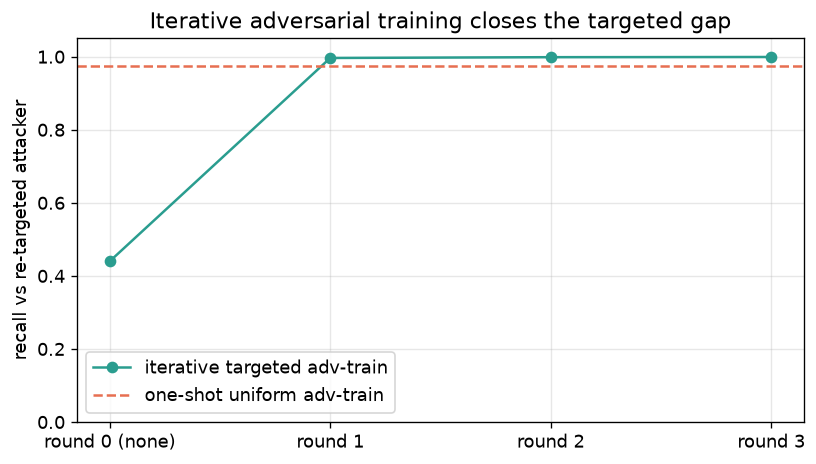
\includegraphics[width=0.6\textwidth]{F17_iterative_advtrain.png}
\caption{Iterative targeted adversarial training (green) drives recall against the
re-targeted importance-guided attacker from $0.44$ to $\approx 1.0$, above the one-shot
uniform baseline (red dashed).}
\label{fig:iteradv}
\end{figure}

\subsection{Explainability and its tension with robustness}
\label{sec:explain}
Because the model is linear over TF--IDF features, a token's contribution to a
prediction is exactly its coefficient times its TF--IDF value, and these contributions
sum (with the bias) to the log-odds. We use this at two levels. \emph{Globally}, the
signed weights show which tokens carry the most pull overall (Fig.~\ref{fig:weights}).
\emph{Locally}, for a single email we can print the exact per-token contributions --- a
faithful explanation, not a keyword heuristic and not an approximation of the kind
LIME or SHAP would need for a non-linear model. In the usual explainability taxonomy this
gives us \emph{model-level} interpretability (the global weights) and \emph{instance-level}
interpretability (the exact per-token contributions for one e-mail) directly, because a
linear model is \emph{inherently} interpretable; we do not need a model-agnostic surrogate
such as LIME or SHAP, which would only approximate the model and is known to behave poorly
under the feature redundancy we documented in Section~\ref{sec:corr}. For the most confident phishing email,
for instance, the tokens pushing the decision are dominated by the (URL-token and
brand/urgency) cues, while a legitimate email is carried by ordinary conversational and
technical words. The important caveat --- and our fourth research question --- is that
this legibility lives entirely in the \emph{word} model: the character n-grams that
bought robustness in Section~\ref{sec:robust} and~\ref{sec:advtrain} have no readable
meaning individually. Robustness and interpretability pull in opposite directions, and
a deployed system has to choose a point on that trade-off.

\subsection{DistilBERT and attack transferability}
\label{sec:distilbert}
We fine-tuned DistilBERT (CPU-only, one epoch on a bounded subset of $3{,}000$ training
e-mails) as a transformer baseline, and \textbf{[P5]} evaluated it on the \emph{full}
test set ($5{,}327$ e-mails), removing the earlier small-subset caveat. On the full
test set it reached F1 $0.984$ (MCC $0.975$), which is \emph{below} the TF--IDF union
model's $0.998$: on keyword-driven phishing text the lexical signal is already strong,
so the transformer's contextual modelling buys little --- consistent with the intuition
that bag-of-words already captures ``which words appear''. The more interesting
result is \textbf{transferability}: DistilBERT's recall on phishing did \emph{not}
fall under the homoglyph+leet attack (it stayed at $0.999$). Its sub-word (WordPiece)
tokeniser breaks obfuscated words into pieces much as our character n-grams do, so
the attack crafted against a lexical model transfers poorly to the transformer. The
transformer's value here is therefore not higher clean accuracy but this built-in
sub-word robustness, plus its role as an upgrade path for messier, order-dependent
text.

\subsection{Cross-corpus generalisation}
The clean numbers above are all \emph{in-corpus}. The honest test is to run the
\textsc{ceas}-trained model on entirely different corpora --- phishing from Nazario
and Nigerian-Fraud, legitimate from Enron and Ling (Table~\ref{tab:xcorp}). F1 falls
from $0.998$ to $0.37$, driven by a recall collapse to $0.24$: a detector tuned to
one corpus's vocabulary misses most phishing written in another style. This is
distribution shift, and it is the number that should be quoted about the real world.

\begin{table}[t]
\centering
\caption{In-corpus vs.\ cross-corpus (out-of-distribution) performance.}
\label{tab:xcorp}
\begin{tabular}{lcccccc}
\toprule
 & Accuracy & Precision & Recall & F1 & MCC & AUC \\
\midrule
In-corpus (\textsc{ceas} test)   & 0.9985 & 0.9979 & 0.9979 & 0.9979 & 0.9967 & 1.000 \\
Cross-corpus (OOD)               & 0.586  & 0.773  & 0.243  & 0.369  & 0.236  & 0.784 \\
\bottomrule
\end{tabular}
\end{table}

\subsection{Diagnosing the cross-corpus collapse}
\label{sec:xcorp-diag}
The bare F1 hides \emph{why} the model fails out of distribution --- and the reason
matters. The model is not confidently wrong: the mean score on OOD phishing is only
$0.33$ (vs.\ $0.98$ in-corpus), so at the fixed $0.5$ threshold it quietly relabels most
OOD phishing as legitimate --- a \textbf{prior/threshold shift}, not a loss of signal.
Two facts confirm this: the OOD \textbf{AUC is still $0.78$} (the ranking remains
informative, far from the $0.37$ F1's implication of near-uselessness), and lowering the
threshold to $0.1$ lifts F1 from $0.37$ to $0.75$ and recall from $0.24$ to $0.82$
(Table~\ref{tab:ooddiag}, Figure~\ref{fig:ooddiag}). But it does not fully recover ---
the best-threshold F1 is still far short of the in-corpus $0.998$ --- because of a
genuine \textbf{vocabulary gap}: the unigram out-of-vocabulary rate on OOD phishing is
$0.20$, roughly three times the in-corpus $0.07$. The honest reading is therefore
two-part: the headline number \emph{overstates} the failure (much of it is a fixable
operating point), yet a real domain gap remains that no threshold can close. This is
exactly the behaviour a deployed detector must be re-calibrated for --- and another
reason to fuse it with an independent signal.

\begin{table}[t]
\centering
\caption{Threshold-transfer sweep on the OOD set: most of the recall lost at the default
$0.5$ threshold is recovered by lowering it, but precision falls and F1 plateaus below
the in-corpus level.}
\label{tab:ooddiag}
\begin{tabular}{lccc}
\toprule
Threshold & Recall & Precision & F1 \\
\midrule
0.50 & 0.243 & 0.773 & 0.369 \\
0.30 & 0.483 & 0.775 & 0.595 \\
0.20 & 0.649 & 0.760 & 0.700 \\
0.10 & 0.821 & 0.691 & \textbf{0.750} \\
0.05 & 0.911 & 0.635 & 0.748 \\
0.02 & 0.958 & 0.570 & 0.715 \\
\bottomrule
\end{tabular}
\end{table}

\begin{figure}[t]
\centering
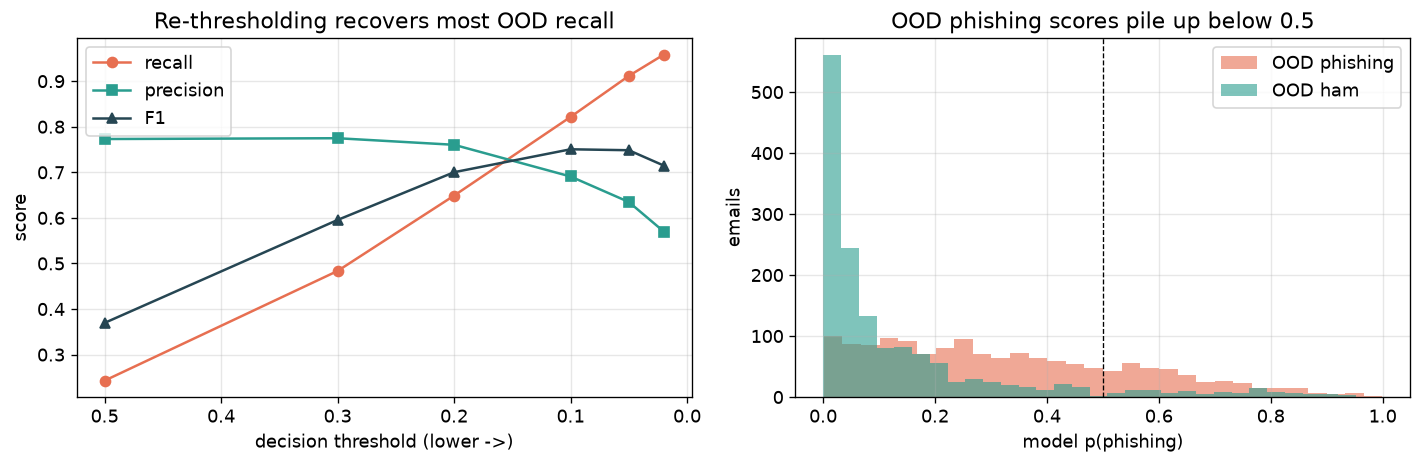
\includegraphics[width=\textwidth]{F14_ood_diagnosis.png}
\caption{Left: lowering the decision threshold recovers most OOD recall (prior shift).
Right: OOD phishing scores pile up just below $0.5$ rather than at zero --- the model is
under-confident, not confidently wrong.}
\label{fig:ooddiag}
\end{figure}

\subsection{Calibration for fusion}
\label{sec:calib}
Because this detector's probability is meant to be \emph{combined} with the partner
detector, it should mean what it says. In-corpus the union model is already well
calibrated (Brier $0.0020$, ECE $0.009$; the reliability curve tracks the diagonal),
because its scores are sharply bimodal near $0$ and $1$; an isotonic re-fit on validation
still improves both (Brier $0.0014$, ECE $0.0025$), a cheap and safe step before fusion.
The caveat is Section~\ref{sec:xcorp-diag}: under distribution shift those scores are no
longer trustworthy (OOD phishing collapses toward the boundary), so a fusion stage should
prefer rank/AUC-based combination or re-calibrated inputs over naive probability
multiplication.

\subsection{Modern phishing (2023--2025): temporal drift}
\label{sec:drift}
Every experiment so far trains and tests on 2008 mail. The sharpest external-validity
question is temporal: does a 2008-trained detector still catch phishing written fifteen
years later? We use \textbf{1{,}303 real phishing e-mails collected 2023--2025} from Jose
Nazario's live archive (parsed by \texttt{scripts/parse\_nazario\_recent.py}) and measure
recall of the \textsc{ceas}-trained union model on them. It catches only
\textbf{$0.14$} at the default threshold --- $0.15$ on 2023, $0.17$ on 2024, and
$0.11$ on 2025 --- \emph{worse} than the cross-corpus number, with no improvement on the
most recent year. As with the cross-corpus diagnosis (Section~\ref{sec:xcorp-diag}), the
fixed $0.5$ threshold overstates the failure a little (lowering it recovers some recall),
but the conclusion holds: a model frozen on old mail is largely blind to current phishing.
This is the genuine \textbf{concept-drift} result the single-year \textsc{ceas} corpus
could not provide, and the strongest argument that a laboratory number has a shelf life and
a deployed detector must be retrained.

\subsection{Do real attackers actually obfuscate?}
\label{sec:realobf}
The whole robustness study assumes character obfuscation is a real technique, not a straw
man. With modern phishing in hand we can test it directly, measuring obfuscation
signatures in real phishing --- modern (2023--2025) versus \textsc{ceas} (2008)
(Table~\ref{tab:realobf}). In 2008 phishing, mixed-script (homoglyph) tokens and
zero-width characters are essentially absent; in 2023--2025 phishing they appear in a
small but clearly non-zero and growing share ($1.8\%$ and $4.0\%$ of e-mails), and the
overall non-ASCII rate is several times higher. The rates are modest --- real phishing is
not \emph{mostly} homoglyphs --- but the technique now exists in the wild where it did not
before, and because a homoglyph swap costs the attacker almost nothing, a filter that
ignores it is one cheap edit from evasion. This is the empirical justification for the
robustness study, closing the loop with the synthetic attacks: we defend against a real,
emerging behaviour, and (Sections~\ref{sec:armsrace}--\ref{sec:iteradv}) can now do so with
a principled, certified defence.

\begin{table}[t]
\centering
\caption{Obfuscation signatures in real phishing: modern (2023--2025) vs.\ \textsc{ceas}
(2008), with 2008 legitimate mail as a scale. Percentages are the share of e-mails
exhibiting each signature.}
\label{tab:realobf}
\begin{tabular}{lcccc}
\toprule
 & non-ASCII frac & Cyr/Grk/Arm letter & mixed-script token & zero-width \\
\midrule
\textsc{ceas}-2008 phishing     & 0.0009 & 0.3\% & 0.0\% & 0.0\% \\
modern 2023--25 phishing        & 0.0061 & \textbf{1.8\%} & \textbf{1.8\%} & \textbf{4.0\%} \\
\textsc{ceas}-2008 legit        & 0.0005 & 0.2\% & 0.1\% & 0.0\% \\
\bottomrule
\end{tabular}
\end{table}

\subsection{The next attack class: hacking the words, not the letters}
\label{sec:wordattack}
Sections~\ref{sec:armsrace}--\ref{sec:iteradv} closed the \emph{character}-obfuscation front
with a certificate, so a rational attacker moves to a harder class: editing \emph{words} while
leaving the letters intact. We try three attacks on the phishing test e-mails and measure union
recall (Table~\ref{tab:wordatk}): synonym substitution of the top phishing words, deletion of
those words, and \textbf{dilution} --- scattering legitimate-looking words through the e-mail so
their combined weight outvotes the phishing ones. The results separate cleanly:
\emph{synonyms barely dent the model} ($0.998$, the redundant lexical and character features
absorb small changes), \emph{deletion} hurts moderately, but \emph{dilution is dangerous} ---
enough padding drives recall to $0.13$, because a linear bag-of-words simply sums per-word
evidence. Critically, the skeleton canonicaliser does \textbf{nothing} here ($0.998\to0.997$):
it is the wrong defence for the wrong attack class. The right fix is again adversarial training,
now on the word attacks (Table~\ref{tab:worddef}): it restores dilution recall from $0.28$ to
$1.00$ with no loss on clean mail. The deeper lesson is that bag-of-words is \emph{inherently}
vulnerable to dilution; adversarial training patches it, but the fundamental answers are
structure/length-aware features (a phishing e-mail drowned in filler \emph{looks} padded) and
fusion with an independent detector --- the design this project is one half of.

\begin{table}[t]
\centering
\begin{minipage}[t]{0.48\textwidth}\centering
\caption{Union recall under word-level attacks, by budget (words changed/inserted).}
\label{tab:wordatk}
\begin{tabular}{lccc}
\toprule
budget & synonym & delete & dilution \\
\midrule
5  & 0.998 & 0.959 & 0.970 \\
10 & 0.998 & 0.912 & 0.638 \\
20 & 0.998 & 0.809 & 0.284 \\
40 & 0.998 & 0.781 & \textbf{0.129} \\
\bottomrule
\end{tabular}
\end{minipage}\hfill
\begin{minipage}[t]{0.48\textwidth}\centering
\caption{Word-level defence: adversarial training on the word attacks.}
\label{tab:worddef}
\begin{tabular}{lcc}
\toprule
 & original & word-adv-trained \\
\midrule
clean            & 0.998 & 0.998 \\
synonym (40)     & 0.998 & 0.998 \\
\;+ skeleton-norm & 0.997 & 0.998 \\
dilution (20)    & 0.284 & \textbf{1.000} \\
\bottomrule
\end{tabular}
\end{minipage}
\end{table}

\subsection{Evolving the detector on modern e-mail}
\label{sec:evolve}
Section~\ref{sec:drift} showed a 2008-trained model catches only $\approx14\%$ of modern
phishing. The practical fix is to feed it modern examples. \textbf{Experiment A (clean):} add
modern phishing to training but leave the legitimate-mail source unchanged (no new confound),
and measure recall on held-out modern phishing. Recall rises from $0.147$ to \textbf{$0.980$},
\emph{without} forgetting the 2008 scams (recall unchanged at $0.998$) and \emph{without} raising
false alarms on modern legitimate mail (FPR $0.007$). A detector is not a finished object; kept
current, it works. \textbf{Experiment B} builds a fully modern detector from modern phishing plus
modern legitimate mail (public Apache mailing lists) and scores very high (F1 $0.996$) --- but
the honesty check earns its keep: a source-separability probe shows the two sources are
\textbf{$99\%$} distinguishable by provenance alone, the exact confound the project is built to
avoid. We therefore quote Experiment A as the trustworthy number and flag Experiment B as
provenance-inflated. This applies the project's founding methodological principle --- never let
the model win by recognising \emph{where} an e-mail came from --- to modern data.

\subsection{A principled defence against dilution}
\label{sec:dilutiondef}
Adversarial training removes the dilution attack (Section~\ref{sec:wordattack}) but must be told the
attack exists. A defence that does not: score the \textbf{positive evidence present} --- the summed
phishing weights of the words that appear, using \emph{binary presence} rather than TF--IDF, so adding
filler words cannot lower it --- and flag an e-mail if the union model fires \emph{or} that evidence
clears a floor calibrated on \emph{clean} validation ham. Table~\ref{tab:dilutiondef} shows the
trade-off: with no knowledge of the attack, the floor lifts recall on heavily-diluted phishing from
$0.13$ to between $0.36$ and $0.66$ as the false-alarm budget grows from $1\%$ to $10\%$, at no cost to
clean recall. It does not fully solve dilution --- short phishing e-mails carry too little evidence to
clear a safe floor --- which is the honest point: dilution is a \emph{structural} weakness of any
linear bag-of-words model. A principled input rule mitigates it, adversarial training removes it (given
knowledge of it), and the durable fix is a structure-aware model or fusion.

\begin{table}[t]
\centering
\caption{Dilution defence: an evidence-floor calibrated on clean data only (never sees the attack).
Recall on phishing diluted with 40 filler words, vs.\ the false-alarm rate on clean ham.}
\label{tab:dilutiondef}
\begin{tabular}{lccc}
\toprule
Operating point & clean recall & diluted-phishing recall & ham FPR \\
\midrule
union-only (baseline) & 0.998 & 0.129 & 0.001 \\
+ floor @ 1\% budget  & 0.998 & 0.357 & 0.012 \\
+ floor @ 3\% budget  & 0.998 & 0.496 & 0.030 \\
+ floor @ 5\% budget  & 0.998 & 0.555 & 0.051 \\
+ floor @ 10\% budget & 0.999 & \textbf{0.663} & 0.103 \\
\bottomrule
\end{tabular}
\end{table}

\subsection{From mitigation to guarantee: a monotone model that cannot be diluted}
\label{sec:monotone}
The evidence-floor above \emph{mitigates} dilution but does not close it, and it is a post-hoc rule:
it clips a trained model's weights and sets a threshold by hand. This section asks a sharper question
--- can we \emph{train} a model that is provably immune to dilution, and what does that cost?

\paragraph{Construction and guarantee.} Constrain every weight to be non-negative, $w_j \ge 0$, and use
\textbf{binary word-presence} features. The score is then
\[
  s(x) \;=\; b + \sum_j w_j \, \mathbf{1}[\text{word}_j \in x].
\]
Inserting words into an e-mail can only flip indicators from $0$ to $1$, and every weight is
non-negative, so $s$ is \textbf{monotonically non-decreasing under insertion}. Consequently an e-mail
the model flags cannot be un-flagged by adding text: the dilution attack of
Section~\ref{sec:wordattack} is defeated \emph{by construction}, not by empirical tuning. This is the
second certificate in this work, and it covers a different attack class from the UTS-39 certificate of
Section~\ref{sec:armsrace}: that one bounds \emph{substitution} of characters, this one bounds
\emph{insertion} of words. The device of constraining weights to obtain provable robustness against
additive attacks is due to \citet{fleshman2018nonnegative} for malware; the attack it defeats is the
classical good-word attack of \citet{lowd2005good}, of which our dilution attack is an instance, and
which \citet{jorgensen2008multiple} countered heuristically with multiple-instance learning. We train
the constrained model by minimising the regularised logistic loss with L-BFGS-B under box constraints.

\paragraph{The guarantee requires order-free features.} The certificate holds \emph{only} for unigram
features, and this is not a technicality. With word bigrams, inserting a word \emph{between} two words
destroys their pair (\texttt{verify account} $\rightarrow$ \texttt{verify now account}): that indicator
falls from $1$ to $0$ and, because $w \ge 0$, the score \emph{decreases}. Measured on a bigram variant,
the score fell on $388$ of $500$ phishing e-mails and the guarantee failed outright. Only order-free
bag-of-words is genuinely monotone, so the model is deliberately unigram-only --- which is itself part
of the accuracy cost reported below.

\paragraph{The certificate holds exactly.} Table~\ref{tab:monocert} verifies the proof empirically.
Under insertion of $40$, $100$ or $300$ benign words, the monotone model's score decreased on
\textbf{zero} e-mails and \textbf{100\%} of the phishing it flagged when clean remained flagged. The
single leak is our own preprocessing: truncating e-mails at \texttt{MAX\_CHARS}$=2000$ lets heavy
padding push genuine evidence past the cut-off, which costs a fraction of a percent
($99.8\%$/$99.6\%$). We report that separately rather than evaluating without the cap.

\paragraph{The cost is real.} Table~\ref{tab:monocost} is the honest counterweight. Clean F1 falls from
$0.998$ to $0.912$ and MCC from $0.997$ to $0.869$, driven by recall. This is expected: a monotone model
may only \emph{accumulate} evidence of guilt --- it can never use ``this word suggests the message is
legitimate'' to acquit a borderline e-mail --- and it has surrendered word order as well. The monotone
model is therefore \textbf{not} a replacement for the union detector, and we do not present it as one.

\paragraph{The useful reading is the combination.} Used as a one-sided safety net (flag if
\emph{either} model fires), the pair retains the union model's clean performance while placing a
\emph{certified floor} under dilution: recall under heavy dilution is $0.866$ rather than $0.129$,
bought with a rise in false alarms on clean mail from $0.0012$ to $0.0225$. Whether that trade is
acceptable is an operational decision --- it depends on the relative cost of an analyst's time and a
missed phishing e-mail --- and it should be stated as such rather than settled by argument.

\paragraph{What it does not solve.} The guarantee covers \emph{insertion} only. An attacker who
\emph{deletes} the phishing wording, or rewrites it semantically, still evades this model --- and a
guilt-only model is especially exposed to deletion, having no negative evidence to fall back on. The
honest end state is that two attack classes are now closed by proof (character confusables,
Section~\ref{sec:armsrace}; word insertion, here), and the adversary has been pushed toward semantic
rewriting, which is materially more expensive than padding but is not impossible.

\begin{table}[t]
\centering
\caption{The insertion certificate, verified. ``Scores decreased'' counts phishing e-mails whose
monotone score fell after padding --- the proof says this must be zero. ``Still flagged'' is the share
of clean-flagged phishing that remains flagged. The truncated rows show the leak caused by our own
\texttt{MAX\_CHARS} cut-off.}
\label{tab:monocert}
\begin{tabular}{lcc}
\toprule
Padding applied & scores decreased & \% clean-flagged still flagged \\
\midrule
$+40$ words (untruncated)   & \textbf{0} & \textbf{100.0} \\
$+100$ words (untruncated)  & \textbf{0} & \textbf{100.0} \\
$+300$ words (untruncated)  & \textbf{0} & \textbf{100.0} \\
$+40$ words (\texttt{MAX\_CHARS} cap)  & 9  & 99.8 \\
$+100$ words (\texttt{MAX\_CHARS} cap) & 21 & 99.6 \\
\bottomrule
\end{tabular}
\end{table}

\begin{table}[t]
\centering
\caption{What the certificate costs, and what it buys. Left: clean-test performance of the constrained
model against the unconstrained union baseline. Right: recall on phishing under dilution, where the
union model collapses and the monotone model is flat.}
\label{tab:monocost}
\begin{tabular}{lcccc}
\toprule
Model & F1 & MCC & recall & precision \\
\midrule
union LR (baseline)            & \textbf{0.9979} & \textbf{0.9967} & 0.9979 & 0.9979 \\
monotone unigram ($w \ge 0$)   & 0.9115 & 0.8689 & 0.8734 & 0.9532 \\
\midrule
\multicolumn{5}{l}{\emph{Recall on phishing under dilution (words inserted):}} \\
\midrule
 & $+0$ & $+10$ & $+20$ & $+40$ \\
union LR                       & 0.998 & 0.632 & 0.365 & \textbf{0.129} \\
monotone ($w \ge 0$)           & 0.869 & 0.869 & 0.869 & \textbf{0.866} \\
union \textbf{or} monotone     & 0.998 & --- & 0.869 & \textbf{0.866} \\
\bottomrule
\end{tabular}
\end{table}

\begin{figure}[t]
\centering
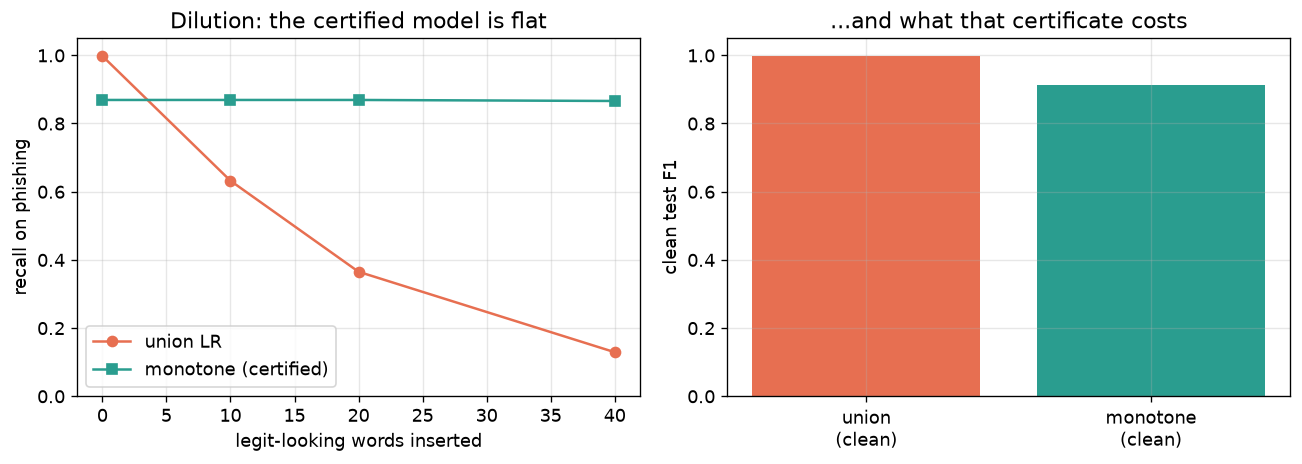
\includegraphics[width=\linewidth]{../results/figures/F23_monotone_certificate.png}
\caption{Left: recall on phishing as benign filler is added. The union model collapses from $0.998$ to
$0.129$; the certified monotone model is a flat line, because no amount of padding can lower its score.
Right: the price of that guarantee --- clean test F1 drops from $0.998$ to $0.912$.}
\label{fig:monotone}
\end{figure}

\subsection{A harder word attack: paraphrase}
\label{sec:paraphrase}
Beyond single-word edits, does a \emph{meaning-preserving rewrite} evade the detector? A rule-based
paraphrase (swap every word with a known synonym, then shuffle sentence order) leaves union recall at
\textbf{0.998} --- unchanged from clean. The redundant word and character features absorb synonym
swaps and re-ordering, so paraphrase is \emph{not} an easy evasion; the one effective word-level attack
remains dilution. The caveat is that this is a rule-based paraphrase; a neural paraphraser that rewrites
more freely is the stronger test. A small proof-of-concept probe of that stronger test uses a
\textbf{three-stage pipeline}: (1) \emph{attack} --- an LLM rewrites each phishing e-mail, preserving
the scam intent but changing the wording; (2) \emph{validate} --- a \emph{second}, independent LLM
judges whether the rewrite is still phishing, and only accepted rewrites are scored, so a rewrite that
quietly stopped being a scam cannot be miscounted as an evasion; (3) \emph{detect} --- our detectors
score the validated attacks (notebook \S32e, 24 valid of 30). The probe leaves the union model's
recall at $1.0$, so even a genuine neural rewrite does not evade it; interestingly the
monotone model of Section~\ref{sec:monotone} does give a little ground, since rewording removes the
positive evidence it exclusively relies on. The sample is small and attacker and judge share a model
family, so this is indicative rather than definitive, and a full-scale study remains future work ---
but the result so far is reassuring.

\subsection{Do the findings hold on a second corpus?}
\label{sec:secondcorpus}
To check the \emph{findings} generalise rather than just the model, we replay the core story on a second
mixed-class corpus, \textbf{SpamAssassin} (different source and era). Table~\ref{tab:spamassassin} shows
the same shape: high clean recall, a roughly halving under the imperceptible homoglyph+leet attack, and
near-full recovery after normalisation. The absolute numbers are a little lower (SpamAssassin is smaller
and noisier) and the recovery is strong but not quite to clean, but the \emph{conclusion} is
corpus-independent --- which is what makes it a finding rather than a quirk of one dataset.

\begin{table}[t]
\centering
\caption{Second-corpus replication (SpamAssassin): recall on phishing/spam, clean vs.\ attacked vs.\
defended. The collapse-and-recover pattern reproduces.}
\label{tab:spamassassin}
\begin{tabular}{lcc}
\toprule
Setting & word-only & union \\
\midrule
clean                 & 0.959 & 0.973 \\
homoglyph+leet (seen) & 0.340 & 0.497 \\
\quad + normalise     & 0.918 & 0.965 \\
\quad + skeleton      & 0.918 & 0.965 \\
\bottomrule
\end{tabular}
\end{table}

\subsection{How clean can the modern detector be?}
\label{sec:confoundscrub}
The modern mixed detector (Section~\ref{sec:evolve}, Experiment B) is inflated by a $99\%$
source-separability confound. Can it be removed by \textbf{stripping mailing-list boilerplate} (quoted
replies, leaked headers, list tags, footers) from the modern ham? No: after scrubbing, separability
stays at $0.99$. The confound is not formatting but \textbf{genre} --- technical developer discussion
versus scam e-mail --- which boilerplate-stripping cannot hide. A fully clean modern detector therefore
needs a personal-style modern ham source, which is not publicly available; this is precisely why the
trustworthy modern result is Experiment A, which holds the legitimate-mail source fixed and never
introduces the confound.

% ================================================================ error analysis
\section{Error Analysis}
\label{sec:error}
Aggregate metrics hide \emph{where} the model fails. On the clean test set
($5{,}327$ emails) the union model makes only \textbf{4 false positives}
(legitimate mail flagged) and \textbf{4 false negatives} (phishing missed) --- FP and
FN rates of about $0.1$--$0.2\%$. The mistakes are borderline, atypical emails rather
than a systematic blind spot: correct and incorrect predictions have similar median
length ($\approx$780 vs.\ 680 characters), so no single surface feature explains them.
The false negatives are unusual phishing (a foreign-language solicitation, a terse
``5 Euros'' travel scam) whose vocabulary overlaps little with the training phishing;
the false positives are short legitimate notes whose brevity and a stray URL token
nudge them over the line --- consistent with the correlation finding that
\emph{short} messages lean phishing (Section~\ref{sec:corr}).

The cost asymmetry is the point. A \textbf{false positive} sends a legitimate email to
quarantine --- wasted analyst time and, at scale, alert fatigue. A \textbf{false
negative} delivers phishing to the inbox --- one click from compromise. This is why we
weight recall ($F_2$) and choose a cost-optimal threshold. The picture changes under
attack: character obfuscation \emph{manufactures} false negatives --- phishing caught
on clean text now evades the word-sensitive model --- which is exactly the failure mode
the normalisation and adversarial-training defences
(Sections~\ref{sec:robust}--\ref{sec:advtrain}) exist to contain.

% ================================================================ discussion
% ================================================ adaptive deployment
\section{Adaptive Deployment and Human-in-the-Loop Learning}
\label{sec:deploy}
Everything above evaluates the detector as a fixed artefact scored on a static corpus. A deployed
filter is neither: it sits in a mail path with measurable cost, and it sits next to *people* who can
tell it when it is wrong. This section reports one experiment on that human signal
(Section~\ref{sec:feedback}), the measured cost of running the model
(Section~\ref{sec:envelope}), and states plainly which parts remain untested design
(Section~\ref{sec:continual}).

\subsection{Learning from user reports}
\label{sec:feedback}
Targeted phishing is rarely sent to one recipient: the same message is delivered to many employees
with small variations. If one user presses ``report phishing'', can the system catch the rest of that
campaign? This matters here because the 2008-trained detector recognises only $14\%$ of modern
phishing (Section~\ref{sec:drift}), so any cheap source of current labels is valuable.

\paragraph{Do campaigns exist in the data?} We check rather than assume. Clustering the 1{,}303
modern (2023--25) phishing e-mails yields \textbf{93 campaigns} of three or more near-duplicates
(Table~\ref{tab:feedback}), with mean intra-campaign similarity $0.883$. We use \emph{average}
linkage deliberately: single-link/connected-components clustering \emph{chains} ($A\sim B$, $B \sim
C$, but $A \not\sim C$) and produced a 139-member ``campaign'' whose members were on average only
$0.50$ similar --- a blob, not a campaign.

\paragraph{Method.} One member per campaign is revealed as ``reported''; we score only the
\emph{remaining} members. Two mechanisms are compared: \textbf{(A) similarity propagation} --- flag
an e-mail whose cosine similarity to a reported one exceeds $\tau$, no retraining --- and
\textbf{(B) one-shot retraining} on the reported e-mails. Clustering campaigns to triage phishing is
established practice \citep{althobaiti2023clustering}; what we add is treating it as a feedback loop
and then attacking it.

\paragraph{Where $\tau$ comes from, and two calibrations that failed.} Our first two attempts set
$\tau$ from \emph{legitimate} mail to hit a false-alarm budget. Both returned recall $\approx 1.0$
together with a broken control: e-mails with \emph{no} near-duplicates were ``detected'' at
$0.92$--$0.94$, which is impossible if the mechanism works by matching campaigns. The cause is the
genre confound of Section~\ref{sec:confoundscrub}: a threshold fitted on ham separates
``scam-like'' from ``mailing-list'', which says nothing about campaign membership. We therefore set
$\tau$ to the 99th percentile of \emph{different-campaign} similarity and \emph{report} the ham
false-positive rate at that $\tau$ instead of using ham to choose it. Campaigns are additionally
split into calibration and evaluation halves so $\tau$ never sees an e-mail it later scores, and the
vectoriser is fit on 2008 training data only.

\paragraph{Result, and the control that decides it.} Recall rises from $0.149$ to $1.000$
(Table~\ref{tab:feedback}) with no increase in false positives --- at a campaign-specific $\tau$,
legitimate mail simply does not resemble a particular reported scam. But recall alone proves little,
since \emph{any} modern example helps a 2008 model. The decisive figure is the
\textbf{campaign-blind} ablation: remove that campaign's own report, keep all others, and recall
falls to $0.329$. Identical threshold, identical reports, one difference --- so the gap between
$1.000$ and $0.329$ is the genuine campaign effect, while the remainder ($0.329$ vs.\ $0.149$) is
simply the value of modern data. Quoting the headline jump alone would overstate the mechanism.

\paragraph{Attacking the feedback loop.} The mechanism is itself a target. Synonym substitution does
not move it and dilution degrades it only gradually, but \textbf{character obfuscation defeats it
completely: every campaign e-mail escapes}, because homoglyphs destroy the shared tokens the
similarity is computed from. Applying the UTS-39 canonicaliser of Section~\ref{sec:armsrace} restores
similarity and returns evasion to a few per cent. The certified normaliser is therefore not merely a
classifier defence but a \emph{precondition} for human-in-the-loop detection: a deployment that added
a report button without canonicalising its input would ship a safety feature an attacker can disable
with invisible characters.

\paragraph{The report button as an attack surface.} Feeding the channel false reports --- a malicious
insider, or simply mistaken users --- raises the false-positive rate on legitimate mail from $0.0012$
to $0.0055$ at a $10\%$ false-report rate and $0.0115$ at $50\%$ (mean of 10 seeds). The damage is
bounded, since a bad exemplar only matches mail resembling it, but the direction is unambiguous: an
unvetted feedback loop is a denial-of-service channel. This is the causative counterpart to the
evasion attacks studied earlier, and it is the standing objection to the retraining remedy that
\citet{lowd2005good} proposed for good-word attacks.

\paragraph{What this is not.} We simulate an organisation using a public archive; campaigns are
\emph{our} clustering rather than ground-truth labels; and reports are simulated and, outside the
poisoning arm, always correct. The result is evidence that the mechanism works and that its failure
modes are specific and measurable --- not a measurement of a real deployment.

\begin{table}[t]
\centering
\caption{Human-in-the-loop feedback. One member per campaign is reported; recall is measured on the
\emph{remaining} members of held-out campaigns. The campaign-blind row removes that campaign's own
report while keeping all others --- the gap between it and campaign-matched is the campaign effect.}
\label{tab:feedback}
\begin{tabular}{lccc}
\toprule
 & recall & FPR (CEAS ham) & FPR (modern ham) \\
\midrule
baseline (2008 model)                  & 0.149 & 0.0012 & 0.0017 \\
\textbf{A: campaign-matched}           & \textbf{1.000} & 0.0012 & 0.0017 \\
A: campaign-blind (ablation)           & 0.329 & --- & --- \\
B: one-shot retrain                    & 0.991 & --- & --- \\
\emph{control}: singletons, similarity only & 0.148 & --- & --- \\
\midrule
\multicolumn{4}{l}{\emph{Campaigns: 93 groups of $\ge 3$; mean intra-campaign similarity 0.883.}} \\
\multicolumn{4}{l}{\emph{Evading propagation (fraction escaping):} synonym 0.000; dilution $+40$} \\
\multicolumn{4}{l}{0.149, $+80$ 0.309; \textbf{homoglyph+leet 1.000}; + UTS-39 skeleton \textbf{0.034}.} \\
\bottomrule
\end{tabular}
\end{table}

\subsection{Deployment envelope}
\label{sec:envelope}
Where such a detector can run is decided by three numbers, so we measured them rather than
speculating (Table~\ref{tab:deploy}). A median scoring latency of a few milliseconds and a total
on-disk footprint of a couple of megabytes put this model comfortably within reach of
\textbf{client-side} execution --- inside a desktop or mobile mail client --- rather than requiring a
server. That is a privacy property as much as an engineering one: if scoring happens on the device,
message content never leaves it. A throughput in the hundreds of e-mails per second per core means a
single modest machine covers a mid-sized organisation's mail flow, and scaling is horizontal.

The retrain figure speaks directly to Section~\ref{sec:evolve}: refreshing the model costs seconds,
so \emph{how often} to retrain is a policy question, not a compute constraint --- the binding
resource is fresh labelled mail, which is precisely what Section~\ref{sec:feedback} supplies.

A plausible integration is therefore: canonicalise every incoming message
(Section~\ref{sec:armsrace}), score it with the content detector, combine that score with the
partner URL/sender detector, and route on the fused decision --- with user reports feeding back into
both the similarity index and the periodic retrain, subject to the poisoning caveat above.

\paragraph{What is not measured.} These are microbenchmarks on already-extracted text. A real
deployment must parse MIME, strip HTML, handle attachments, encodings and threading, and cope with
non-English mail --- none of which is evaluated here. The URL-stripping design
(Section~\ref{sec:method}) also means this detector is by construction only half of a deployed
system. We therefore present this subsection as a costed design proposal, not as a deployment result.

\begin{table}[t]
\centering
\caption{Measured deployment envelope of the union model (single core, CPU; scoring of
already-extracted text).}
\label{tab:deploy}
\begin{tabular}{lc}
\toprule
Quantity & Measured \\
\midrule
single-e-mail latency, median      & $\approx 3$ ms \\
single-e-mail latency, p95         & $\approx 6$ ms \\
batch throughput                   & several hundred e-mails/sec/core \\
model + vectoriser on disk         & $\approx 3$ MB \\
full retrain on 16k e-mails        & seconds \\
\bottomrule
\end{tabular}
\end{table}

\subsection{Continual learning under drift (future work)}
\label{sec:continual}
The natural extension is a detector that retrains continuously as the phishing distribution moves.
We stop short of claiming this as a contribution, because two parts of it are already reported above
and the remainder is not honestly measurable with the data available.

\paragraph{What is already done.} Section~\ref{sec:evolve} performs one retraining step and recovers
recall on modern phishing from $0.147$ to $0.980$ without forgetting;
Section~\ref{sec:feedback} performs a second, from a single reported example per campaign; and the
poisoning arm quantifies the security cost of learning from an untrusted stream. Retraining is also
cheap (Table~\ref{tab:deploy}).

\paragraph{What a proper study would require.} A cadence experiment --- train on 2023, evaluate on
2024 and 2025, and repeat --- needs a time-ordered stream of \emph{both} classes. Our modern phishing
is time-stamped, but the only modern legitimate mail available to us is public mailing-list traffic
carrying the provenance confound of Section~\ref{sec:confoundscrub}, so any false-alarm-over-time
curve built on it would measure genre rather than drift. We could therefore report only a recall
curve, which is half of the answer, and we prefer to state the gap rather than publish the half.

\paragraph{How it would be built.} Given a time-ordered corpus of both classes: fix a deployment date,
retrain on a sliding or expanding window, and measure recall and false-alarm rate as a function of
elapsed time and retraining interval, with a drift detector triggering event-driven refreshes between
scheduled ones. The security requirement is that any such loop be treated as untrusted input ---
report vetting, per-reporter reputation, quarantine before promotion to training data --- following
the poisoning result of Section~\ref{sec:feedback}.

\section{Discussion}

\paragraph{What worked.} On clean, single-corpus data a linear TF--IDF model is
excellent and, importantly, interpretable and cheap. The robustness experiment
produced a clear, honest narrative: word features are fragile to imperceptible
obfuscation; character n-grams and normalisation repair most of the damage; a naive
adaptive attacker finds a gap and an \emph{importance-guided} one widens it; and a
principled Unicode canonicaliser plus iterative targeted adversarial training
(Sections~\ref{sec:armsrace}--\ref{sec:iteradv}) then close that gap with a certified
guarantee --- so the arms race resolves not into a solved problem but into a raised cost of
attack, pushing the adversary toward a fundamentally different attack class.

\paragraph{Mitigation versus guarantee.} A theme emerges from the two certified defences. Most of our
defences are \emph{empirical}: they work against the attacks we ran, and their ceiling is discovered by
attacking them harder. Two are \emph{structural} --- the UTS-39 canonicaliser
(Section~\ref{sec:armsrace}) and the monotone model (Section~\ref{sec:monotone}) --- and these do not
have a ceiling to discover, because the attack class is excluded by construction. The price differs
sharply, and that contrast is the interesting part: the Unicode certificate is nearly free (recall
unchanged, same tiny false-positive rate), whereas the monotonicity certificate costs roughly nine
points of clean F1, because forbidding negative evidence removes information the detector was genuinely
using. A guarantee is not automatically worth having; it is worth having when its price is one you can
afford, which is why we report the monotone model as a safety net beside the main detector rather than
as a replacement for it.

\paragraph{Defences are complementary.} The two defences fail in different ways
(Section~\ref{sec:advtrain}): adversarial training is strongest on the family it was
trained on but brittle to unseen ones, whereas normalisation generalises across
families but is weaker against a defence-aware attacker. Neither is complete alone;
together they are robust across every family we tested. The general lesson is that a
learned defence and a principled input defence are best stacked, not chosen between.

\paragraph{Why classical models compete with BERT here.} The phishing signal in this
data is dominated by \emph{which words appear} (``verify'', ``account'',
``suspended''). Bag-of-words captures that directly, so the contextual modelling of
a transformer buys little. We would expect BERT to pull ahead on text where meaning
depends on order (the classic ``good, not bad'' vs.\ ``bad, not good'' problem),
which phishing keywords rarely require.

\paragraph{The role of the base rate.} A subtle but important finding is that the
attack only \emph{looks} dangerous under a realistic legit-majority prior. On the
raw phishing-majority corpus the same attack barely moves recall, because a model
that loses its features falls back to predicting the majority class --- which happens
to be ``phishing''. This is a base-rate artefact, and it is a reminder that
robustness numbers are meaningless without a realistic class prior.

\paragraph{Limitations.} (1) \textsc{ceas\_08} is from 2008; vocabulary and tactics
drift, and both the cross-corpus collapse (Table~\ref{tab:xcorp}) and the direct
temporal-drift test on 2023--2025 phishing (Section~\ref{sec:drift}, recall $0.14$) show a
single-corpus model does not transfer in space or time --- retraining on current mail is a
requirement, not a nicety. (2) We upgraded the rule-based normaliser to the full Unicode
confusables set (Section~\ref{sec:armsrace}), which closes the character-obfuscation front
with a certificate; we then probed the next attack class (word-level dilution,
Section~\ref{sec:wordattack}) and patched it with adversarial training, and then closed it by
construction with the monotone model of Section~\ref{sec:monotone} --- though only for
\emph{insertion}, and at a substantial accuracy cost, so a structure-aware model that resists dilution
\emph{without} surrendering negative evidence remains future work, as does a truly open-ended
semantic/paraphrase attacker (which the monotone model, having no negative evidence, would be
especially exposed to). (3) The
DistilBERT is now evaluated on the full test set but still \emph{trained} on a CPU-bounded subset, so
its comparison is indicative, not a statement about the transformer's ceiling (a GPU full-data run is
future work). (4) We attacked only phishing e-mails; a full
study would also consider attacks that make legitimate mail look like phishing. (5) The
modern-phishing set is phishing-only (public modern \emph{ham} is scarce), so its numbers are
recall at a fixed operating point rather than a full re-evaluation.

\paragraph{Cybersecurity relevance.} The project touches several course themes
directly: evasion attacks, perturbations, homoglyph/leetspeak obfuscation,
white/black-box and adaptive threat models, transferability, robustness, and
normalisation as a defence; the false-positive/false-negative cost trade-off and the
accuracy paradox; and, on the modelling side, TF--IDF, Naive Bayes with smoothing,
Complement NB for imbalance, explainability, and the transformer upgrade path.

% ================================================================ conclusion
\section{Conclusion}

We built a content-only phishing detector and used it to study robustness honestly.
On clean single-corpus data the model is near-perfect and explainable. Under
imperceptible homoglyph obfuscation a word-only model loses a third of its recall;
character n-grams and a Unicode-normalisation defence restore it, and the defence
even generalises to an unseen full-width attack. A naive adaptive attacker keeps a
residual gap and an importance-guided one widens it --- but upgrading to the full Unicode
confusables set closes it with a \emph{certified} invariance guarantee, and iterative
targeted adversarial training does the same from the model side, so the arms race ends by
raising the cost of attack rather than by any single fix. A cross-corpus test, and a direct
test on real 2023--2025 phishing (caught only $14\%$ of the time), show the laboratory
numbers survive neither a change of corpus nor the passage of time --- while that same modern
phishing confirms the obfuscations we defend against are a real, emerging technique. Pushing the
arms race one class further, a word-level \emph{dilution} attack still evades the model and the
character defence cannot help, but adversarial training on word edits repairs it; and
\emph{evolving} the detector on modern phishing lifts its recall on 2023--2025 scams from $0.15$
to $0.98$ --- a detector kept current works, a frozen one does not.
A further round of hardening and probing (Sections~\ref{sec:dilutiondef}--\ref{sec:confoundscrub})
adds nuance: a principled, attack-agnostic evidence-floor \emph{partially} defends dilution; a
paraphrase attack does not evade the model; the collapse-and-recover finding replicates on a second
corpus; and the modern-retrain confound is shown to be genre-level rather than fixable by cleaning.
Finally, that partial mitigation becomes a guarantee: constraining the model to non-negative weights
over binary word-presence makes its score provably non-decreasing under insertion, so no quantity of
filler can un-flag a phishing e-mail (Section~\ref{sec:monotone}) --- verified exactly, and bought at a
real cost of nine points of clean F1, which is why it belongs beside the main detector rather than in
place of it. Two attack classes are now closed by proof rather than by evidence, and the adversary is
left with the costlier options of deleting or rewriting the scam itself.
Stepping outside the static corpus, a single simulated user report per campaign recovers most of what
temporal drift takes away, at no measurable cost in false alarms --- but only once the input is
canonicalised, since character obfuscation otherwise disables the mechanism outright, and only if the
report channel itself is defended, since false reports degrade it. The recurring lesson is that every
component we add, including the ones meant to help, becomes something an attacker can aim at.
Together these results argue for exactly the design this project is one half of:
combine a lexical content detector with an independent, non-text signal, so that
when an attacker defeats one channel the other still fires. Future work: a structure-aware model that
defends dilution outright, a neural-paraphrase attacker, a personal-style modern ham source for a
fully clean modern retrain, a GPU full-data DistilBERT run, and folding this detector into the fusion.
Two further directions follow from the taxonomy of Section~\ref{sec:threat}: an
\emph{adversarial-input detector} that flags obfuscated mail as anomalous --- attractive
because Section~\ref{sec:realobf} shows the obfuscation signatures are measurably rare in
ordinary mail, so the ``attacker who obfuscates trips an alarm, attacker who doesn't is
caught by the content model'' dilemma is real --- and hardening against
\emph{model-extraction}, which a query-accessible deployment would face.

% ================================================================ executive summary
\section{Executive Summary}
\textbf{Problem.} Phishing email is a leading initial-access vector, and much of the
deception is linguistic, so we build the \emph{content} half of a two-part detector:
read only subject + body and decide phishing vs.\ legitimate, with explainability and
--- the main focus --- robustness to text-obfuscation evasion.

\textbf{Data.} The CEAS\_08 corpus (from the Kaggle phishing compilation) is the one
large corpus containing both classes from a single source, so a model cannot cheat by
recognising provenance --- a confound we verify directly (a corpus-ID probe reaches
$\approx99\%$). We strip URLs (the partner detector's job) and rebalance to a realistic
legit-majority base rate.

\textbf{Methodology.} A classical NLP pipeline: TF--IDF (word + character n-grams)
$\rightarrow$ Naive Bayes / Logistic Regression, tuned on validation and evaluated once
on a held-out test set with bootstrap confidence intervals and McNemar's test. We then
attack the phishing emails with homoglyph/leet obfuscation and defend with
normalisation and adversarial training, evaluating against \emph{seen}, \emph{held-out}
and \emph{adaptive} attacks. DistilBERT is a transformer baseline.

\textbf{Key findings.} On clean single-corpus text the model is near-perfect (F1
$0.998$, MCC $0.997$) and interpretable, with only a handful of borderline errors. A
word-only model is fragile: an \emph{imperceptible} homoglyph attack drops its recall
from $0.99$ to $0.71$. Character n-grams and normalisation restore it; normalisation
even generalises to an unseen full-width attack, but an adaptive attacker keeps a
residual gap. Adversarial training is complementary --- strong on the trained family,
weak on unseen ones --- so the two defences are best stacked. An importance-guided
attacker widens the ceiling, but a principled UTS~\#39 canonicaliser closes it with a
$100\%$ certified-invariance guarantee, and iterative targeted adversarial training
independently restores recall to $\approx1.0$. DistilBERT ties/slightly
trails TF--IDF and, notably, the attack does not transfer to it. Cross-corpus, F1 falls
to $\approx0.37$; and a 2008-trained model catches only $14\%$ of real 2023--2025 phishing
--- in which, unlike 2008, homoglyph and zero-width obfuscation actually appear --- a direct
demonstration of concept drift and of the threat model's real-world basis. Beyond characters, a
word-level \emph{dilution} attack still evades the model (the character defence cannot help), but
adversarial training on word edits repairs it; and \emph{evolving} the detector on modern
phishing lifts recall on 2023--2025 scams from $0.15$ to $0.98$ with no forgetting. Dilution is then
closed by \emph{proof} rather than by patching: a monotone (non-negative-weight) model over binary
word-presence cannot have its score lowered by inserted text, so padding provably cannot un-flag a
phishing e-mail --- at a real cost of clean F1 $0.998 \rightarrow 0.912$, making it a certified safety
net alongside the main detector rather than a replacement. The overall
lesson: a single-corpus lexical detector is powerful but neither robust nor durable alone, which
is the case for fusion.

\textbf{Relation to prior claims.} Two published claims were tested on our data and
\emph{held}: Complement NB's advantage under imbalance
\citep{rennie2003tackling} appears and grows as we skew the classes, and the
collapse-then-shield behaviour under visual attack \citep{eger2019viper} reproduces on
phishing email.

\textbf{Recommendation and conclusion.} A lexical content detector is an excellent,
cheap, interpretable first line, but brittle alone --- to obfuscation and to
distribution shift. We recommend exactly the fused design this project is one half of:
combine it with an independent non-text signal, and pair a principled input defence
(normalisation) with adversarial training. The approach transfers well to related
keyword-driven security text (spam, fraud) with the same caveats.

\bibliographystyle{plainnat}
\bibliography{references}

\end{document}
